\documentclass[aspectratio=169]{beamer}

\usepackage{tikz}
\usetikzlibrary{arrows.meta}    % for Stealth arrow tips
\usetikzlibrary{positioning}    % for "below=of node" syntax
\usetikzlibrary{shapes.geometric} % for diamond shape
% ============================================================
% STANFORD COLOR PALETTE
% ============================================================
\usepackage{xcolor}
\definecolor{cardinal}{HTML}{8C1515}
\definecolor{sandstone}{HTML}{D2C295}
\definecolor{lightsand}{HTML}{F9F6EF}
\definecolor{coolgrey}{HTML}{4D4F53}

% ============================================================
% THEME: minimal
% ============================================================
\usetheme{default}
\usecolortheme{default}

\setbeamercolor{structure}{fg=cardinal}
\setbeamercolor{frametitle}{fg=cardinal}
\setbeamercolor{title}{fg=cardinal}
\setbeamercolor{subtitle}{fg=coolgrey}
\setbeamercolor{author}{fg=coolgrey}
\setbeamercolor{date}{fg=coolgrey}
\setbeamercolor{institute}{fg=coolgrey}
\setbeamercolor{normal text}{fg=black, bg=white}
\setbeamercolor{item}{fg=cardinal}
\setbeamercolor{subitem}{fg=sandstone}
\setbeamercolor{block title}{fg=white, bg=cardinal}
\setbeamercolor{block body}{bg=lightsand}

\setbeamertemplate{navigation symbols}{}
\setbeamertemplate{footline}{}

\setbeamerfont{frametitle}{size=\large, series=\bfseries}
\setbeamerfont{title}{size=\Large, series=\bfseries}

% ============================================================
% PACKAGES
% ============================================================
\usepackage{amsmath, amssymb}
\usepackage{graphicx}
\usepackage{booktabs}

% ============================================================
% METADATA
% ============================================================
\title{cCKF: Calibrated Combinatorial Kalman Filter}
\subtitle{Replacing Heuristic Cuts with Learned, Calibrated Decisions}
\author{Matthew Musson}
\institute{Stanford University}
\date{August 28, 2026}

% ============================================================
% DOCUMENT
% ============================================================
\begin{document}

\begin{frame}
  \titlepage
\end{frame}

\begin{frame}{Outline}
  \tableofcontents
\end{frame}

\section{Motivation}

\subsection{The $\chi^2$ Cut}
\begin{frame}{What ACTS Does Today}
  \begin{columns}
    \begin{column}{0.5\textwidth}
      \begin{itemize}
        \item ACTS reconstructs tracks in three steps:
        \begin{enumerate}
          \item Seeding
          \item The CKF
          \item Ambiguity Resolution
        \end{enumerate}
        \item The CKF cuts on the $\chi^2$ value of a candidate hit which is a weighted version of the hits residual with respect to predicted measurement, weighted by the covariance of the Kalman filter
      \end{itemize}
    \end{column}

    \begin{column}{0.5\textwidth}
      \begin{align}     
        C_k^{k-1} &= FC_{k-1}^{k-1}F^T + Q_k\\ 
        S_k &= H_k C_k^{k-1} H_k^\top + R_k \\
        \hat m_k &= H_k\vec x  \\ 
         r &= h_k - \hat{m_k} \\
        \chi^2 &= r^\top S^{-1} r 
      \end{align}
    \end{column}
  \end{columns}
\end{frame}
                                    
\subsection{Why It Fails}
\begin{frame}{The CKF Algorithm}

    \begin{columns}

    \begin{column}{0.6\textwidth}
        \begin{itemize}
            \item The CKF applies a uniform cut to all hits, selecting those within a $\chi^2$ threshold 
            \item The CKF Branches on these hits up to $\text{numMeasurementsCutOff}$ 
            \item If there are no measurements within $\text{ChiSquaredCutOffMeasurement}$ it checks for hits within chi2CutOffOutlier branching on those instead 
            \item If no hits are within chi2CutOffOutlier then the CKF logs a hole
            \item Finally the CKF prunes branches which exceed a max count of holes, outliers, or sequential holes, as well as branches with a $\chi^2_{tot}$ or $p_T$ which fail thresholds
        \end{itemize}
    \end{column}

    \begin{column}{0.4\textwidth}
        \resizebox{!}{0.85\textheight}{%
            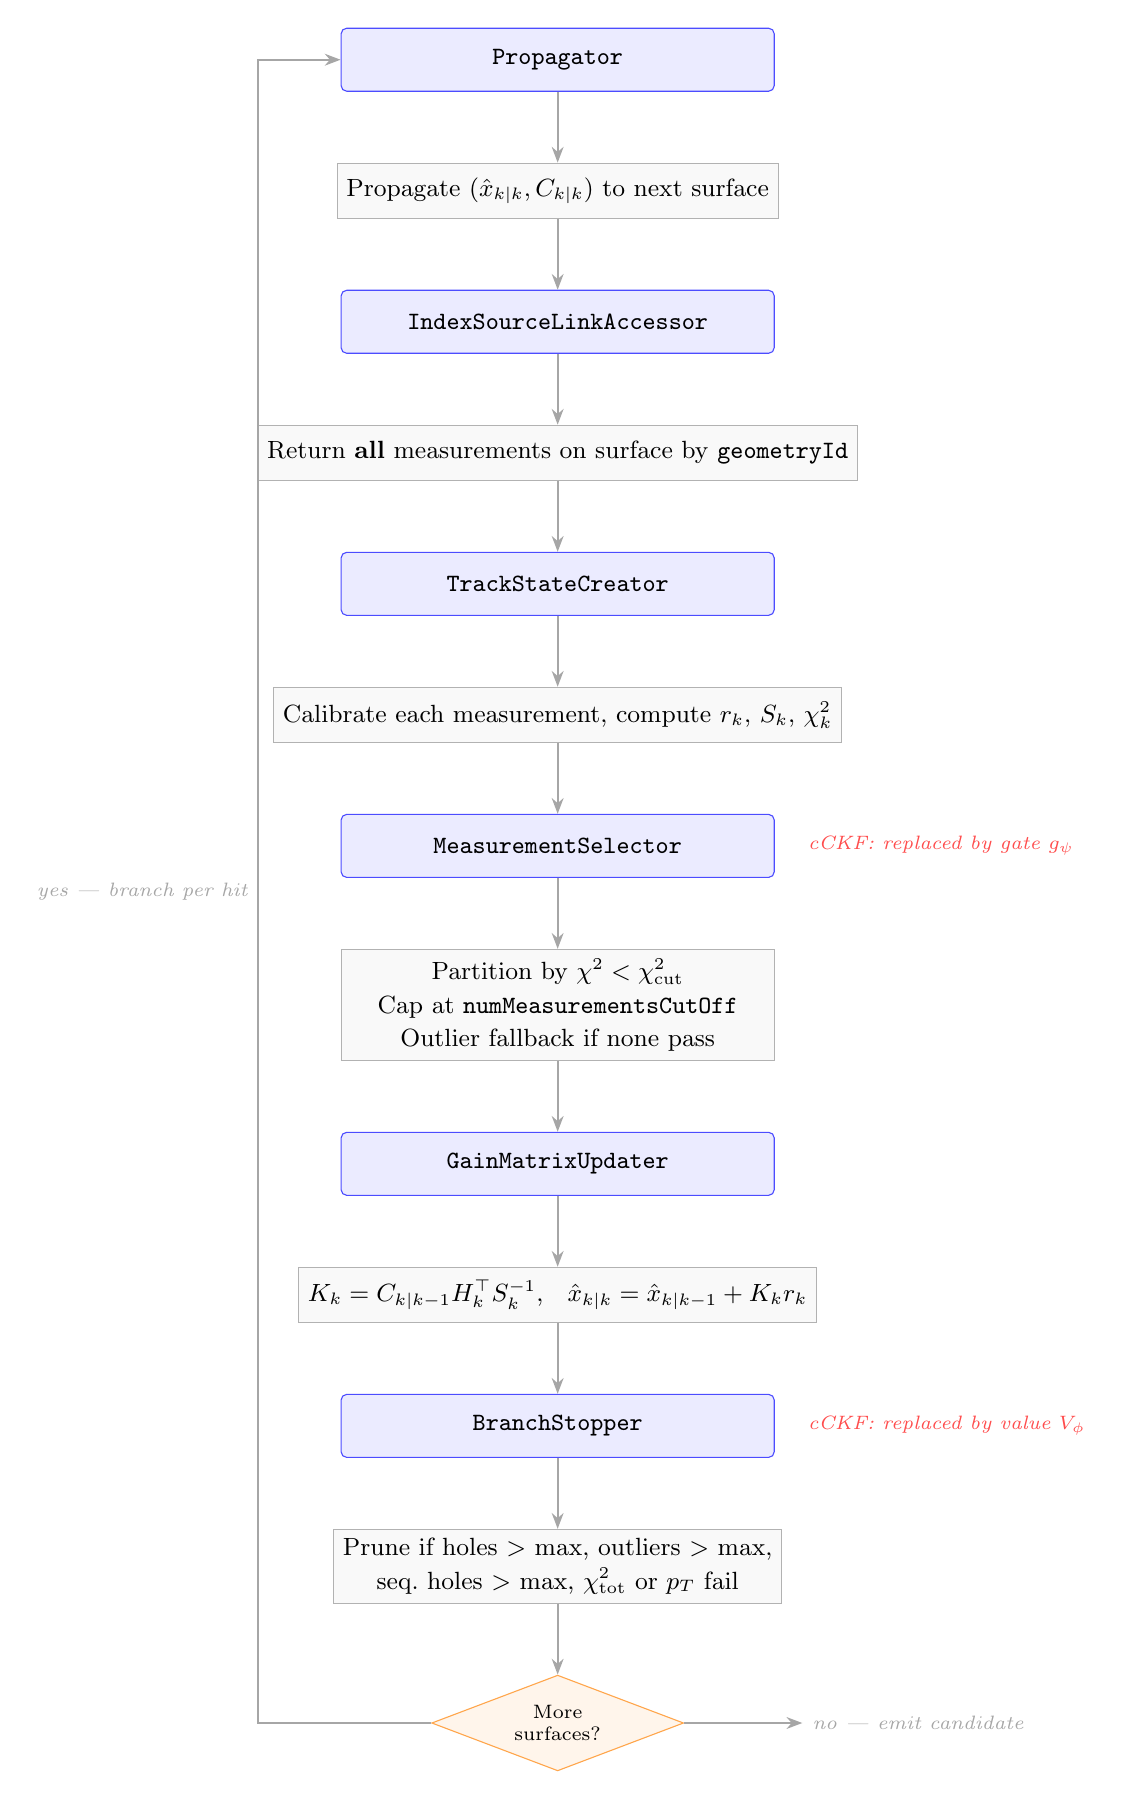
\begin{tikzpicture}[
                node distance=0.9cm,
                every node/.style={font=\small},
                class/.style={rectangle, draw=blue!70, fill=blue!8, 
                    minimum width=5.5cm, minimum height=0.8cm, 
                    rounded corners=2pt, align=center, font=\small\ttfamily},
                action/.style={rectangle, draw=gray!60, fill=gray!5,
                    minimum width=5.5cm, minimum height=0.7cm,
                    align=center, font=\small},
                decision/.style={diamond, draw=orange!70, fill=orange!8,
                    minimum width=3.2cm, minimum height=0.8cm,
                    align=center, font=\scriptsize, aspect=2.5},
                arrow/.style={-{Stealth[length=2mm]}, thick, draw=gray!70},
                label/.style={font=\scriptsize\itshape, text=gray!70},
            ]
            
            % Nodes
            \node[class] (prop) {Propagator};
            \node[action, below=of prop] (prop_act) {Propagate $(\hat{x}_{k|k}, C_{k|k})$ to next surface};
            
            \node[class, below=of prop_act] (slac) {IndexSourceLinkAccessor};
            \node[action, below=of slac] (slac_act) {Return \textbf{all} measurements on surface by \texttt{geometryId}};
            
            \node[class, below=of slac_act] (tsc) {TrackStateCreator};
            \node[action, below=of tsc] (tsc_act) {Calibrate each measurement, compute $r_k$, $S_k$, $\chi^2_k$};
            
            \node[class, below=of tsc_act] (ms) {MeasurementSelector};
            \node[action, below=of ms] (ms_act) {
                Partition by $\chi^2 < \chi^2_\text{cut}$\\[1pt]
                Cap at \texttt{numMeasurementsCutOff}\\[1pt]
                Outlier fallback if none pass
            };
            
            \node[class, below=of ms_act] (gmu) {GainMatrixUpdater};
            \node[action, below=of gmu] (gmu_act) {$K_k = C_{k|k-1} H_k^\top S_k^{-1}$, \; $\hat{x}_{k|k} = \hat{x}_{k|k-1} + K_k r_k$};
            
            \node[class, below=of gmu_act] (bs) {BranchStopper};
            \node[action, below=of bs] (bs_act) {
                Prune if holes $>$ max, outliers $>$ max,\\[1pt]
                seq.\ holes $>$ max, $\chi^2_\text{tot}$ or $p_T$ fail
            };
            
            \node[decision, below=of bs_act] (done) {More\\surfaces?};
            
            % Arrows
            \draw[arrow] (prop) -- (prop_act);
            \draw[arrow] (prop_act) -- (slac);
            \draw[arrow] (slac) -- (slac_act);
            \draw[arrow] (slac_act) -- (tsc);
            \draw[arrow] (tsc) -- (tsc_act);
            \draw[arrow] (tsc_act) -- (ms);
            \draw[arrow] (ms) -- (ms_act);
            \draw[arrow] (ms_act) -- (gmu);
            \draw[arrow] (gmu) -- (gmu_act);
            \draw[arrow] (gmu_act) -- (bs);
            \draw[arrow] (bs) -- (bs_act);
            \draw[arrow] (bs_act) -- (done);
            
            % Loop back
            \draw[arrow] (done.west) -- ++(-2.2,0) |- node[label, near start, left] {yes — branch per hit} (prop.west);
            \draw[arrow] (done.east) -- ++(1.5,0) node[label, right] {no — emit candidate};
            
            % Side annotations
            \node[label, right=0.3cm of ms] (cckf_note) {\color{red!70}cCKF: replaced by gate $g_\psi$};
            \node[label, right=0.3cm of bs] (cckf_note2) {\color{red!70}cCKF: replaced by value $V_\phi$};
            
            \end{tikzpicture}
            }%
     \end{column}
    \end{columns}
\end{frame}

\begin{frame}{Miscalibration}
\begin{columns}
    \begin{column}{0.5\textwidth}
      \begin{itemize}
        \item This algorithm is insufficient in three main ways
        \begin{enumerate}
          \item It is myopic with respect to detector occupancy - there is no account for local hit density (like in a jet core)
          \item The decision boundary exists only in $\chi^2$ which is a compression of significantly more relevant signal ($\eta$, cluster features, etc.) 
          \item The branch pruning is heuristic, not taking into account per measurement features
        \end{enumerate}
        \item Aa naive cut on $\chi^2$ is blind to non-guassian processes like hard scatters through detector material, requiring a learned discriminator
      \end{itemize}
    \end{column}

    \begin{column}{0.5\textwidth}
    $$ p(y = 1 |x) \approx \frac{1}{\sqrt{2\pi\det(S_k)}} \exp\left[-\frac{1}{2}r_k^TS_k^{-1}r_k \right]$$
      \begin{figure}
          \centering
          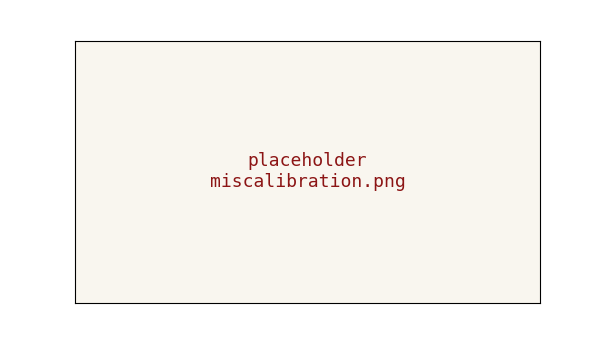
\includegraphics[width=0.7\linewidth]{miscalibration.png}
          \caption{Miscalibration given implied Gaussian Probability}
          \label{fig:placeholder}
      \end{figure}
    \end{column}
  \end{columns}
\end{frame}

\begin{frame}{Window Failure Rate}

\begin{figure}
    \centering
    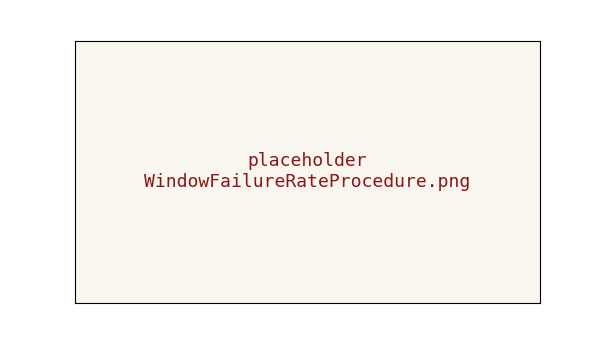
\includegraphics[width=1\linewidth]{WindowFailureRateProcedure.png}
    \caption{Computing Window Failure Rate}
    \label{fig:placeholder}
\end{figure}
  
\end{frame}

\begin{frame}{Window Failure Rate}
\begin{itemize}
    \item We can see that hits fall out of the $S_k$ weighted search window with accumulated material (data collected from optimized CKF config on ColliderML) 
\end{itemize}
\begin{figure}
    \centering
    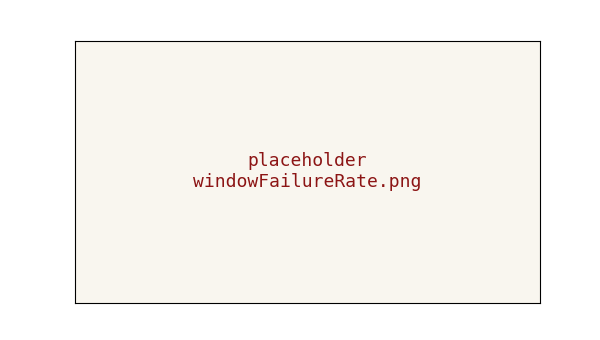
\includegraphics[width=0.9\linewidth]{windowFailureRate.png}
    \caption{Window failure rate across $\eta$, stratified by sensor type and seed purity, for window sizes $n = 3$ to $10$}
    \label{fig:placeholder}
\end{figure}
  
\end{frame}

\section{Method}

\subsection{Gate Function $g_\psi$}

\begin{frame}{Learned Gate $g_\psi$}
  \begin{columns}
    \begin{column}{0.5\textwidth}
      \textbf{Answers:} Is this hit from the same particle as the branch?

      \vspace{0.3cm}
      \textbf{Feature vector} (26-dim):
      \begin{itemize}
        \item Residual $r_k$ (2D), Cholesky of $S_k$ (3), $\chi^2_k$
        \item Cluster: size, charge, second moments $\sigma_{uu}, \sigma_{uv}, \sigma_{vv}$
        \item Normalized cluster: $\kappa_u, \kappa_v, \tilde{Q}$
        \item Occupancy $n_\text{window}$
        \item Context: $\eta$, $q/p$, step $k$, $X/X_0$
        \item Sensor: pitch$_u$, pitch$_v$, thickness, is\_pixel
        \item Branch history: $n_\text{hits}$, $n_\text{holes}$, $n_\text{seq\_holes}$
      \end{itemize}

      \vspace{0.3cm}
      \textbf{Replaces:} $\chi^2 < \chi^2_\text{cut}$
    \end{column}

    \begin{column}{0.5\textwidth}
      % Architecture block diagram
      \centering
      \resizebox{!}{0.5\textheight}{%
      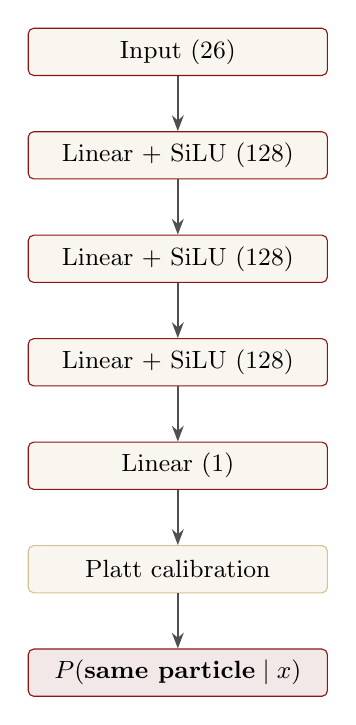
\begin{tikzpicture}[
        node distance=0.7cm,
        block/.style={rectangle, draw=cardinal, fill=lightsand,
          minimum width=3.8cm, minimum height=0.6cm,
          rounded corners=2pt, align=center, font=\small},
        arrow/.style={-{Stealth[length=2mm]}, thick, draw=coolgrey},
      ]
        \node[block] (input) {Input (26)};
        \node[block, below=of input] (h1) {Linear + SiLU (128)};
        \node[block, below=of h1] (h2) {Linear + SiLU (128)};
        \node[block, below=of h2] (h3) {Linear + SiLU (128)};
        \node[block, below=of h3] (logit) {Linear (1)};
        \node[block, below=of logit, draw=sandstone, fill=sandstone!15]
          (platt) {Platt calibration};
        \node[block, below=of platt, draw=cardinal, fill=cardinal!10,
          font=\small\bfseries] (out) {$P(\text{same particle} \mid x)$};

        \draw[arrow] (input) -- (h1);
        \draw[arrow] (h1) -- (h2);
        \draw[arrow] (h2) -- (h3);
        \draw[arrow] (h3) -- (logit);
        \draw[arrow] (logit) -- (platt);
        \draw[arrow] (platt) -- (out);
      \end{tikzpicture}
      }%

      \vspace{0.4cm}
      % Loss function
      \textbf{Loss:} Unweighted BCE
      $$ \mathcal L=-\frac{1}{N}\sum_i \left[ y_i \log \hat{p}_i + (1-y_i)\log(1-\hat{p}_i) \right]$$

    \end{column}
  \end{columns}
\end{frame}

\begin{frame}{Incidence angle and expected charge}

\begin{figure}
    \centering
    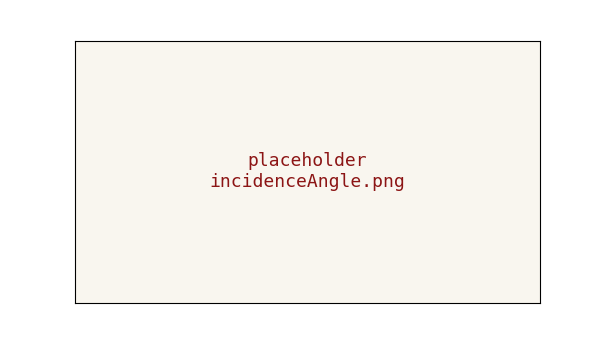
\includegraphics[width=1\linewidth]{incidenceAngle.png}
    \caption{How the incidence angle and expected pitch are calculated}
    \label{fig:placeholder}
\end{figure}
    
\end{frame}

\begin{frame}{Defining a Majority Particle}
\begin{columns}
    \begin{column}{0.5\textwidth}
        \begin{itemize}
            \item In order for the gate function to be well defined we need to define a branch's majority particle
            \item In building seeding triplets there are three cases to consider
            \begin{itemize}
                \item The triplet is pure, containing (3/3) hits from the same particle 
                \item The triplet has a majority, but one wrong hit, with purity (2/3)
                \item The triplet is a mix of 3 different particles 
            \end{itemize}
            \item We exclude case 3 and train only on seeds with a majority particle --- training a set of models on just pure triplets (which experience significantly lower window failure rates) 
        \end{itemize}
    \end{column}
    \begin{column}{0.5\textwidth}
      \centering
      \resizebox{!}{0.75\textheight}{%
      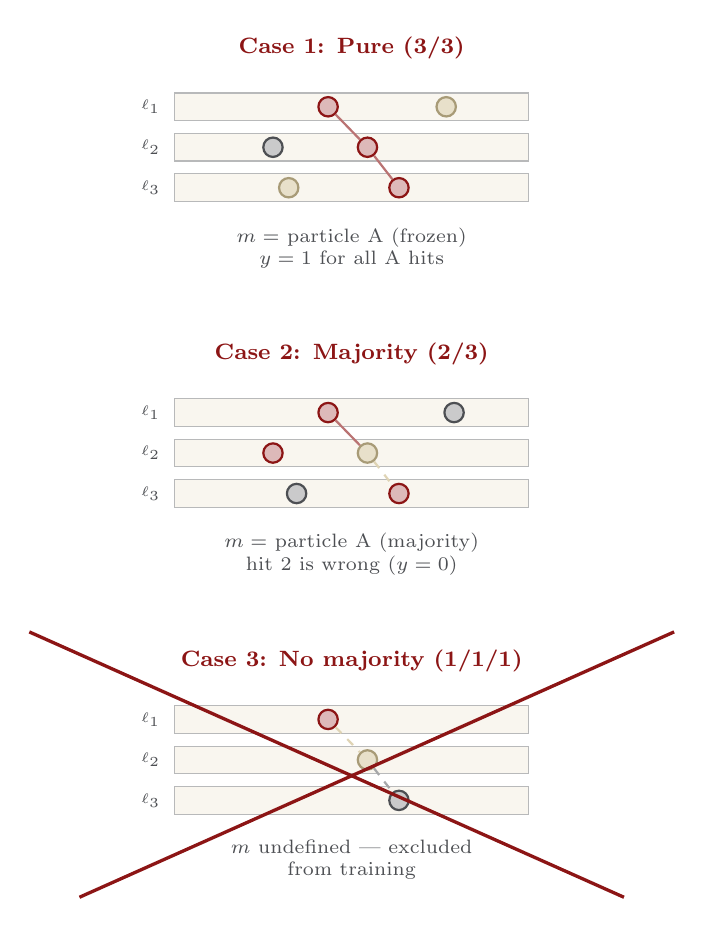
\begin{tikzpicture}[
        node distance=0.4cm,
        layer/.style={draw=coolgrey!40, minimum width=4.5cm, minimum height=0.35cm,
          fill=lightsand, font=\tiny\color{coolgrey}},
        hit/.style={circle, minimum size=7pt, inner sep=0pt, thick},
        hitA/.style={hit, draw=cardinal, fill=cardinal!30},
        hitB/.style={hit, draw=sandstone!80!black, fill=sandstone!50},
        hitC/.style={hit, draw=coolgrey, fill=coolgrey!30},
        conn/.style={thick, draw=cardinal!60},
        connB/.style={thick, draw=sandstone!70, dashed},
        connC/.style={thick, draw=coolgrey!50, dashed},
        caselbl/.style={font=\footnotesize\bfseries, text=cardinal},
        annot/.style={font=\scriptsize, text=coolgrey, align=center},
      ]

      % === Case 1: Pure (3/3) ===
      \node[caselbl] (c1lbl) {Case 1: Pure (3/3)};
      \node[layer, below=0.3cm of c1lbl] (c1L1) {};
      \node[layer, below=0.15cm of c1L1] (c1L2) {};
      \node[layer, below=0.15cm of c1L2] (c1L3) {};
      \node[font=\tiny\color{coolgrey}, left=0.05cm of c1L1] {$\ell_1$};
      \node[font=\tiny\color{coolgrey}, left=0.05cm of c1L2] {$\ell_2$};
      \node[font=\tiny\color{coolgrey}, left=0.05cm of c1L3] {$\ell_3$};

      \node[hitA] (c1h1) at ([xshift=-0.3cm]c1L1.center) {};
      \node[hitA] (c1h2) at ([xshift=0.2cm]c1L2.center) {};
      \node[hitA] (c1h3) at ([xshift=0.6cm]c1L3.center) {};
      % Distractors
      \node[hitB] at ([xshift=1.2cm]c1L1.center) {};
      \node[hitC] at ([xshift=-1.0cm]c1L2.center) {};
      \node[hitB] at ([xshift=-0.8cm]c1L3.center) {};

      \draw[conn] (c1h1) -- (c1h2);
      \draw[conn] (c1h2) -- (c1h3);

      \node[annot, below=0.2cm of c1L3] (c1a) {%
        $m = $ particle A (frozen)\\
        $y=1$ for all A hits};

      % === Case 2: Majority (2/3) ===
      \node[caselbl, below=0.7cm of c1a] (c2lbl) {Case 2: Majority (2/3)};
      \node[layer, below=0.3cm of c2lbl] (c2L1) {};
      \node[layer, below=0.15cm of c2L1] (c2L2) {};
      \node[layer, below=0.15cm of c2L2] (c2L3) {};
      \node[font=\tiny\color{coolgrey}, left=0.05cm of c2L1] {$\ell_1$};
      \node[font=\tiny\color{coolgrey}, left=0.05cm of c2L2] {$\ell_2$};
      \node[font=\tiny\color{coolgrey}, left=0.05cm of c2L3] {$\ell_3$};

      \node[hitA] (c2h1) at ([xshift=-0.3cm]c2L1.center) {};
      \node[hitB] (c2h2) at ([xshift=0.2cm]c2L2.center) {};
      \node[hitA] (c2h3) at ([xshift=0.6cm]c2L3.center) {};
      % Distractors
      \node[hitC] at ([xshift=1.3cm]c2L1.center) {};
      \node[hitA] at ([xshift=-1.0cm]c2L2.center) {};
      \node[hitC] at ([xshift=-0.7cm]c2L3.center) {};

      \draw[conn] (c2h1) -- (c2h2);
      \draw[connB] (c2h2) -- (c2h3);

      \node[annot, below=0.2cm of c2L3] (c2a) {%
        $m = $ particle A (majority)\\
        hit 2 is wrong ($y=0$)};

      % === Case 3: No majority ===
      \node[caselbl, below=0.7cm of c2a] (c3lbl) {Case 3: No majority (1/1/1)};
      \node[layer, below=0.3cm of c3lbl] (c3L1) {};
      \node[layer, below=0.15cm of c3L1] (c3L2) {};
      \node[layer, below=0.15cm of c3L2] (c3L3) {};
      \node[font=\tiny\color{coolgrey}, left=0.05cm of c3L1] {$\ell_1$};
      \node[font=\tiny\color{coolgrey}, left=0.05cm of c3L2] {$\ell_2$};
      \node[font=\tiny\color{coolgrey}, left=0.05cm of c3L3] {$\ell_3$};

      \node[hitA] (c3h1) at ([xshift=-0.3cm]c3L1.center) {};
      \node[hitB] (c3h2) at ([xshift=0.2cm]c3L2.center) {};
      \node[hitC] (c3h3) at ([xshift=0.6cm]c3L3.center) {};

      \draw[connB] (c3h1) -- (c3h2);
      \draw[connC] (c3h2) -- (c3h3);

      \node[annot, below=0.2cm of c3L3] (c3a) {%
        $m$ undefined --- excluded\\
        from training};

      % Strike-through
      \draw[very thick, cardinal] ([xshift=-1.8cm, yshift=0.1cm]c3lbl.north west)
        -- ([xshift=1.8cm, yshift=-0.1cm]c3a.south east);
      \draw[very thick, cardinal] ([xshift=1.8cm, yshift=0.1cm]c3lbl.north east)
        -- ([xshift=-1.8cm, yshift=-0.1cm]c3a.south west);

      \end{tikzpicture}
      }%
    \end{column}
\end{columns}
\end{frame}


\begin{frame}{Feature Extraction Mechanics}
\centering
\resizebox{0.95\textwidth}{!}{%
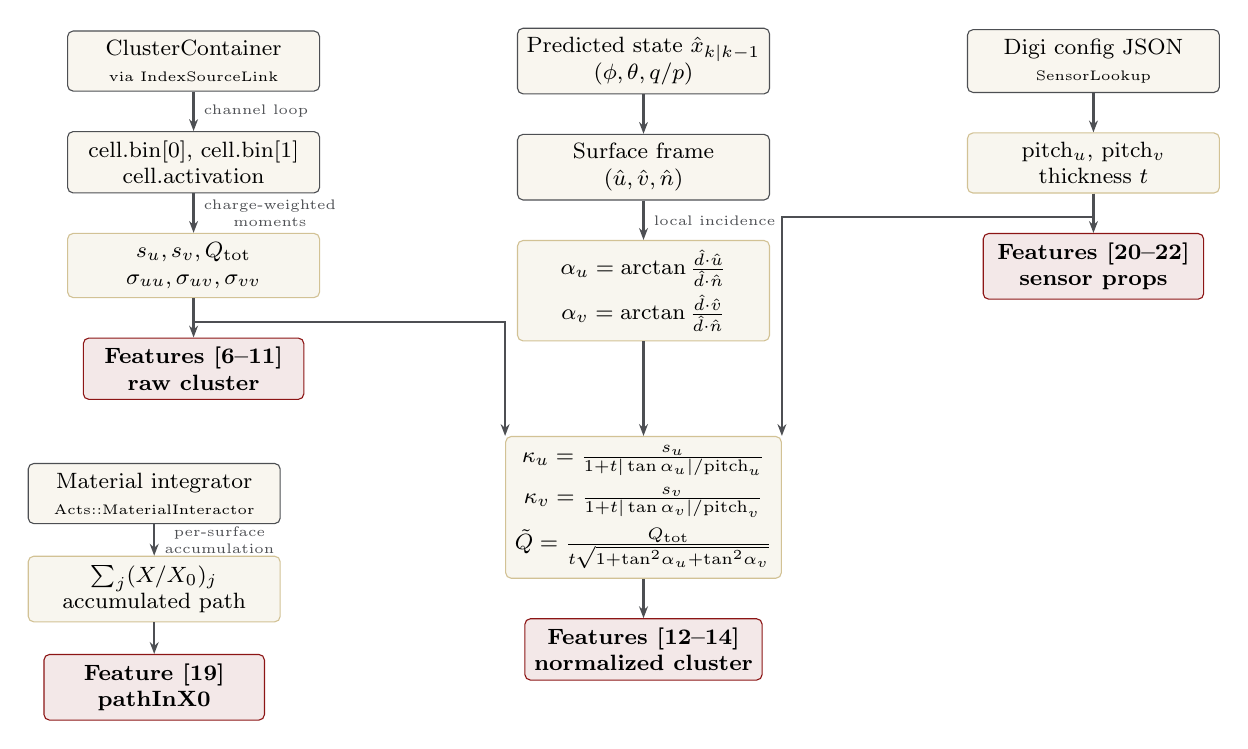
\begin{tikzpicture}[
  node distance=0.4cm and 0.6cm,
  source/.style={rectangle, draw=coolgrey, fill=lightsand,
    minimum width=3.2cm, minimum height=0.55cm,
    rounded corners=2pt, align=center, font=\footnotesize},
  derived/.style={rectangle, draw=sandstone, fill=sandstone!15,
    minimum width=3.2cm, minimum height=0.55cm,
    rounded corners=2pt, align=center, font=\footnotesize},
  feature/.style={rectangle, draw=cardinal, fill=cardinal!10,
    minimum width=2.8cm, minimum height=0.5cm,
    rounded corners=2pt, align=center, font=\footnotesize\bfseries},
  arrow/.style={-{Stealth[length=1.5mm]}, thick, draw=coolgrey},
  label/.style={font=\tiny\color{coolgrey}, align=center},
]
% === Column 1: Cluster features ===
\node[source] (cluster) {ClusterContainer\\{\tiny via IndexSourceLink}};
\node[source, below=0.5cm of cluster] (cells) {cell.bin[0], cell.bin[1]\\cell.activation};
\node[derived, below=0.5cm of cells] (raw) {$s_u, s_v, Q_\text{tot}$\\$\sigma_{uu}, \sigma_{uv}, \sigma_{vv}$};
\node[feature, below=0.5cm of raw] (rawfeat) {Features [6--11]\\raw cluster};
\draw[arrow] (cluster) -- node[right, label] {channel loop} (cells);
\draw[arrow] (cells) -- node[right, label] {charge-weighted\\moments} (raw);
\draw[arrow] (raw) -- (rawfeat);

% === Column 2: Incidence angles ===
\node[source, right=2.5cm of cluster] (predict) {Predicted state $\hat{x}_{k|k-1}$\\$(\phi, \theta, q/p)$};
\node[source, below=0.5cm of predict] (surface) {Surface frame\\$(\hat{u}, \hat{v}, \hat{n})$};
\node[derived, below=0.5cm of surface] (angles) {$\alpha_u = \arctan\frac{\hat{d}\cdot\hat{u}}{\hat{d}\cdot\hat{n}}$\\[2pt]$\alpha_v = \arctan\frac{\hat{d}\cdot\hat{v}}{\hat{d}\cdot\hat{n}}$};
\draw[arrow] (predict) -- (surface);
\draw[arrow] (surface) -- node[right, label] {local incidence} (angles);

% === Column 3: Sensor geometry ===
\node[source, right=2.5cm of predict] (sensor) {Digi config JSON\\{\tiny SensorLookup}};
\node[derived, below=0.5cm of sensor] (props) {pitch$_u$, pitch$_v$\\thickness $t$};
\node[feature, below=0.5cm of props] (sensorfeat) {Features [20--22]\\sensor props};
\draw[arrow] (sensor) -- (props);
\draw[arrow] (props) -- (sensorfeat);

% === Merge: Normalized cluster features ===
\node[derived, below=1.2cm of angles] (normalized) {%
  $\kappa_u = \frac{s_u}{1 + t|\tan\alpha_u|/\text{pitch}_u}$\\[3pt]
  $\kappa_v = \frac{s_v}{1 + t|\tan\alpha_v|/\text{pitch}_v}$\\[3pt]
  $\tilde{Q} = \frac{Q_\text{tot}}{t\sqrt{1+\tan^2\!\alpha_u+\tan^2\!\alpha_v}}$
};
\node[feature, below=0.5cm of normalized] (normfeat) {Features [12--14]\\normalized cluster};
\draw[arrow] (raw.south) -- ++(0,-0.3) -| (normalized.north west);
\draw[arrow] (angles) -- (normalized);
\draw[arrow] (props.south) -- ++(0,-0.3) -| (normalized.north east);
\draw[arrow] (normalized) -- (normfeat);

% === Bottom left: pathInX0 ===
\node[source, below=0.8cm of rawfeat, xshift=-0.5cm] (material) {Material integrator\\{\tiny Acts::MaterialInteractor}};
\node[derived, below=0.4cm of material] (pathacc) {$\sum_j (X/X_0)_j$\\accumulated path};
\node[feature, below=0.4cm of pathacc] (pathfeat) {Feature [19]\\pathInX0};
\draw[arrow] (material) -- node[right, label] {per-surface\\accumulation} (pathacc);
\draw[arrow] (pathacc) -- (pathfeat);
\end{tikzpicture}
}%
\end{frame}
    


\subsection{Value Function $V_\phi$}

\begin{frame}{Learned Value Function $V_\phi$}
  \begin{columns}
    \begin{column}{0.5\textwidth}
      \textbf{Answers:} Will this branch complete to a matched track?

      \vspace{0.3cm}
      \textbf{Feature vector} (11-dim):
      \begin{itemize}
        \item Gate log-odds (accumulated)
        \item $\chi^2_\text{tot}$, mean $\chi^2$ per hit
        \item $n_\text{hits}$, $n_\text{holes}$, $n_\text{seq\_holes}$
        \item $\eta$, $q/p$, $p_T$
        \item Step $k$, $X/X_0$ accumulated
      \end{itemize}

      \vspace{0.3cm}
      \textbf{Target:} $V^{\pi^\dagger}$ (truth-greedy rollout)
      \begin{align*}
        % \text{completeness} &= \frac{n_\text{correct} + n_\text{findable}}{N_\text{true}} \\
        % \text{purity} &= \frac{n_\text{correct} + n_\text{findable}}{n_\text{correct} + n_\text{wrong} + n_\text{findable}} \\
        V^{\pi^\dagger} &= \min(\text{completeness},\; \text{purity})
      \end{align*}

      \vspace{0.1cm}
      \textbf{Replaces:} hole/branch caps
    \end{column}

    \begin{column}{0.5\textwidth}
      % Architecture block diagram
      \centering
      \resizebox{!}{0.45\textheight}{%
      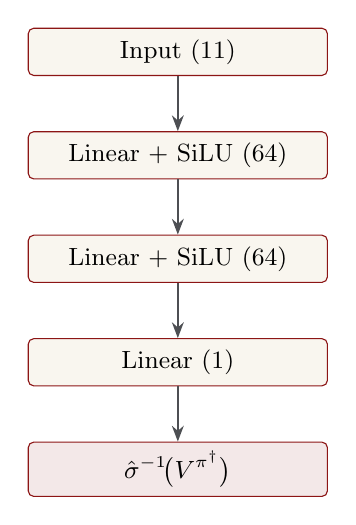
\begin{tikzpicture}[
        node distance=0.7cm,
        block/.style={rectangle, draw=cardinal, fill=lightsand,
          minimum width=3.8cm, minimum height=0.6cm,
          rounded corners=2pt, align=center, font=\small},
        arrow/.style={-{Stealth[length=2mm]}, thick, draw=coolgrey},
      ]
        \node[block] (input) {Input (11)};
        \node[block, below=of input] (h1) {Linear + SiLU (64)};
        \node[block, below=of h1] (h2) {Linear + SiLU (64)};
        \node[block, below=of h2] (logit) {Linear (1)};
        \node[block, below=of logit, draw=cardinal, fill=cardinal!10,
          font=\small\bfseries]
          (out) {$\hat{\sigma}^{-1}\!\big(V^{\pi^\dagger}\big)$};

        \draw[arrow] (input) -- (h1);
        \draw[arrow] (h1) -- (h2);
        \draw[arrow] (h2) -- (logit);
        \draw[arrow] (logit) -- (out);
      \end{tikzpicture}
      }%

      \vspace{0.5cm}
      % Loss function
      \textbf{Loss:} Soft-target BCE
      $$\mathcal{L} = -\frac{1}{N}\sum_i \left[ v_i \log \hat{v}_i + (1-v_i)\log(1-\hat{v}_i) \right]$$
      where $v_i = V^{\pi^\dagger}_i \in [0,1]$ is a soft label.


     
    \end{column}
  \end{columns}
\end{frame}

\begin{frame}{Three Tiers of the Value Function}
\begin{columns}
    \begin{column}{0.5\textwidth}
        \begin{itemize}
            \item The value function predicts if a branch will complete to a DM-matched track 
            \item Three tiers of oracle rollout, each a weaker upper bound:
            \begin{itemize}
                \item Tier 1 ($V^*$): knows the true trajectory everywhere, even beyond CKF surfaces
                \item Tier 2 ($V^{\pi^\dagger}_\text{reprop}$): picks correct hits on CKF surfaces, re-propagates from them (fixes corrupted Kalman state)
                \item Tier 3 ($V^{\pi^\dagger}$): picks best available hit on each CKF surface, no re-propagation
            \end{itemize}
            \item Tier 3 is the tightest bound the CKF can achieve without modifying the propagator
        \end{itemize}
    \end{column}
        \begin{column}{0.5\textwidth}
      \centering
      \resizebox{!}{0.85\textheight}{%
      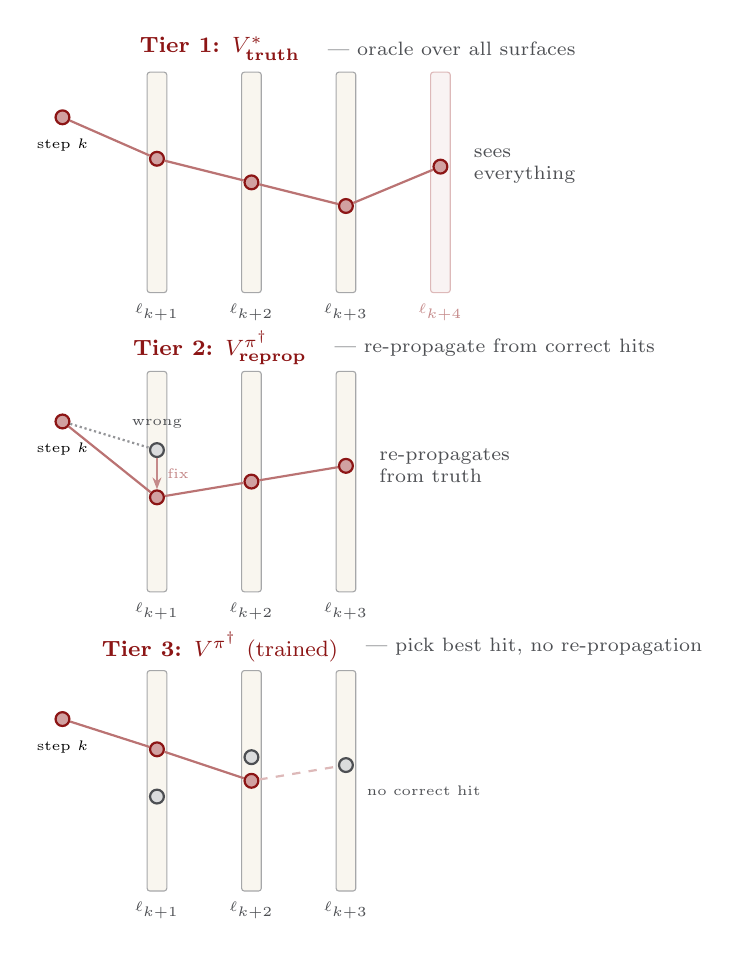
\begin{tikzpicture}[
        node distance=0.3cm,
        surface/.style={draw=coolgrey!50, minimum width=0.25cm,
          minimum height=2.8cm, fill=lightsand, rounded corners=1pt},
        hit/.style={circle, minimum size=5pt, inner sep=0pt, thick},
        hitT/.style={hit, draw=cardinal, fill=cardinal!40},
        hitW/.style={hit, draw=coolgrey, fill=coolgrey!20},
        traj/.style={thick, cardinal!60},
        trajD/.style={thick, cardinal!30, dashed},
        ckfpath/.style={thick, coolgrey!60, densely dotted},
        arrow/.style={-{Stealth[length=1.5mm]}, thick, draw=coolgrey},
        tierlbl/.style={font=\footnotesize\bfseries, text=cardinal},
        annot/.style={font=\scriptsize, text=coolgrey, align=left},
      ]

      % === Tier 1 ===
      \node[tierlbl] (t1lbl) at (0,0) {Tier 1: $V^*_\text{truth}$};
      \node[annot, right=0.1cm of t1lbl] {--- oracle over all surfaces};

      \node[hitT, below=0.5cm of t1lbl, xshift=-2cm] (t1s) {};
      \node[font=\tiny, below=0.05cm of t1s] {step $k$};

      \foreach \i/\x in {1/-0.8, 2/0.4, 3/1.6} {
        \node[surface] (t1surf\i) at (\x, -1.7) {};
        \node[font=\tiny\color{coolgrey}, below=0.01cm of t1surf\i] {$\ell_{k+\i}$};
      }
      \node[hitT] (t1h1) at (-0.8, -1.4) {};
      \node[hitT] (t1h2) at (0.4, -1.7) {};
      \node[hitT] (t1h3) at (1.6, -2.0) {};
      \node[surface, draw=cardinal!30, fill=cardinal!5] (t1surf4) at (2.8, -1.7) {};
      \node[font=\tiny\color{cardinal!50}, below=0.01cm of t1surf4] {$\ell_{k+4}$};
      \node[hitT] (t1h4) at (2.8, -1.5) {};

      \draw[traj] (t1s) -- (t1h1) -- (t1h2) -- (t1h3) -- (t1h4);
      \node[annot, right=0.2cm of t1h4] {sees\\everything};

      % === Tier 2 (shifted down more) ===
      \node[tierlbl] (t2lbl) at (0, -3.8) {Tier 2: $V^{\pi^\dagger}_\text{reprop}$};
      \node[annot, right=0.1cm of t2lbl] {--- re-propagate from correct hits};

      \node[hitT, below=0.5cm of t2lbl, xshift=-2cm] (t2s) {};
      \node[font=\tiny, below=0.05cm of t2s] {step $k$};

      \foreach \i/\x in {1/-0.8, 2/0.4, 3/1.6} {
        \node[surface] (t2surf\i) at (\x, -5.5) {};
        \node[font=\tiny\color{coolgrey}, below=0.01cm of t2surf\i] {$\ell_{k+\i}$};
      }
      \node[hitW] (t2w1) at (-0.8, -5.1) {};
      \draw[ckfpath] (t2s) -- (t2w1);
      \node[font=\tiny\color{coolgrey}, above=0.05cm of t2w1] {wrong};

      \node[hitT] (t2c1) at (-0.8, -5.7) {};
      \node[hitT] (t2c2) at (0.4, -5.5) {};
      \node[hitT] (t2c3) at (1.6, -5.3) {};
      \draw[traj] (t2s) -- (t2c1);
      \draw[traj] (t2c1) -- (t2c2) -- (t2c3);

      \draw[arrow, cardinal!50] (t2w1) -- (t2c1)
        node[midway, right, font=\tiny\color{cardinal}] {fix};

      \node[annot, right=0.2cm of t2c3] {re-propagates\\from truth};

      % === Tier 3 (shifted down more) ===
      \node[tierlbl] (t3lbl) at (0, -7.6)
        {Tier 3: $V^{\pi^\dagger}$ \normalfont\footnotesize(trained)};
      \node[annot, right=0.1cm of t3lbl] {--- pick best hit, no re-propagation};

      \node[hitT, below=0.5cm of t3lbl, xshift=-2cm] (t3s) {};
      \node[font=\tiny, below=0.05cm of t3s] {step $k$};

      \foreach \i/\x in {1/-0.8, 2/0.4, 3/1.6} {
        \node[surface] (t3surf\i) at (\x, -9.3) {};
        \node[font=\tiny\color{coolgrey}, below=0.01cm of t3surf\i] {$\ell_{k+\i}$};
      }
      \node[hitT] (t3c1) at (-0.8, -8.9) {};
      \node[hitW] (t3cw1) at (-0.8, -9.5) {};
      \node[hitT] (t3c2) at (0.4, -9.3) {};
      \node[hitW] (t3cw2) at (0.4, -9.0) {};
      \node[hitW] (t3cw3) at (1.6, -9.1) {};
      \node[font=\tiny\color{coolgrey}, below right=0.1cm of t3cw3] {no correct hit};

      \draw[traj] (t3s) -- (t3c1) -- (t3c2);
      \draw[trajD] (t3c2) -- (t3cw3);

      % \node[annot, right=0.2cm of t3cw3, yshift=-0.3cm]
      %   {stuck with\\CKF state};

      % % Inequality (pushed down)
      % \node[font=\normalsize, text=cardinal] at (0.4, -10.8)
      %   {$V^{\pi^\dagger} \;\leq\; V^{\pi^\dagger}_\text{reprop}
      %    \;\leq\; V^*_\text{truth}$};

      \end{tikzpicture}
      }%
    \end{column}
\end{columns}
\end{frame}

\subsection{Training}
\begin{frame}{Training Six Models}
\begin{columns}
    \begin{column}{0.5\textwidth}
        \begin{itemize}
            \item We want to examine the performance of the gate function when trained on pure triplets or all majority defined seeds 
            \item We also want to examine the difference between the tier 2 and tier 3 value functions 
            \item Thus we are left to train six different models 
            \item We run all of them on the test split to examine distribution shift when exposed to seeds which have purity of (2/3) and (3/3) 
        \end{itemize}
    \end{column}
    \begin{column}{0.5\textwidth}
      \centering
      \resizebox{0.95\columnwidth}{!}{%
      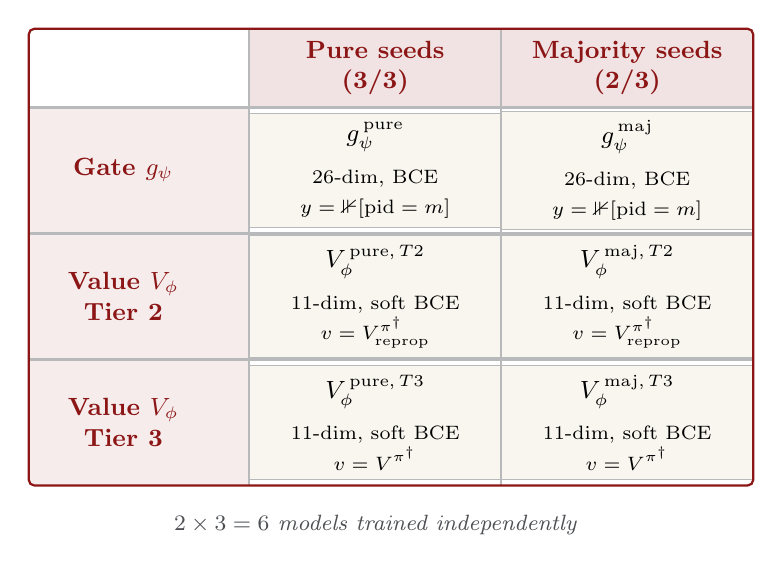
\begin{tikzpicture}[
        cell/.style={rectangle, minimum width=3.2cm, minimum height=1.4cm,
          align=center, font=\small},
        header/.style={cell, fill=cardinal!12, font=\small\bfseries,
          text=cardinal, minimum height=0.9cm},
        rowlbl/.style={cell, fill=cardinal!8, font=\small\bfseries,
          text=cardinal, minimum width=2.4cm, minimum height=1.4cm},
        data/.style={cell, draw=coolgrey!40, fill=lightsand,
          minimum width=3.2cm, minimum height=1.4cm},
        corner/.style={cell, fill=white, minimum width=2.4cm,
          minimum height=0.9cm},
      ]

     % Row label backgrounds (fill the full cell area)
      \fill[cardinal!8, rounded corners=1pt]
        (-1.2, -0.5) rectangle (1.6, -2.1);
      \fill[cardinal!8, rounded corners=1pt]
        (-1.2, -2.1) rectangle (1.6, -3.7);
      \fill[cardinal!8, rounded corners=1pt]
        (-1.2, -3.7) rectangle (1.6, -5.3);

      % Column header backgrounds
      \fill[cardinal!12, rounded corners=1pt]
        (1.6, 0.5) rectangle (4.8, -0.5);
      \fill[cardinal!12, rounded corners=1pt]
        (4.8, 0.5) rectangle (8.0, -0.5);

      % Corner
      \node[corner] (corner) at (0, 0) {};

      % Column headers
      \node[header] (h1) at (3.2, 0) {Pure seeds\\(3/3)};
      \node[header] (h2) at (6.4, 0) {Majority seeds\\(2/3)};

      % Row 1: Gate
      \node[rowlbl] (r1) at (0, -1.3) {Gate $g_\psi$};
      \node[data] (g1) at (3.2, -1.3) {$g_\psi^{\,\text{pure}}$\\[4pt]
        {\scriptsize 26-dim, BCE}\\
        {\scriptsize $y=\mathbb{1}[\text{pid}=m]$}};
      \node[data] (g2) at (6.4, -1.3) {$g_\psi^{\,\text{maj}}$\\[4pt]
        {\scriptsize 26-dim, BCE}\\
        {\scriptsize $y=\mathbb{1}[\text{pid}=m]$}};

      % Row 2: Value Tier 2
      \node[rowlbl] (r2) at (0, -2.9) {Value $V_\phi$\\Tier 2};
      \node[data] (v21) at (3.2, -2.9) {$V_\phi^{\,\text{pure},\,T2}$\\[4pt]
        {\scriptsize 11-dim, soft BCE}\\
        {\scriptsize $v = V^{\pi^\dagger}_\text{reprop}$}};
      \node[data] (v22) at (6.4, -2.9) {$V_\phi^{\,\text{maj},\,T2}$\\[4pt]
        {\scriptsize 11-dim, soft BCE}\\
        {\scriptsize $v = V^{\pi^\dagger}_\text{reprop}$}};

      % Row 3: Value Tier 3
      \node[rowlbl] (r3) at (0, -4.5) {Value $V_\phi$\\Tier 3};
      \node[data] (v31) at (3.2, -4.5) {$V_\phi^{\,\text{pure},\,T3}$\\[4pt]
        {\scriptsize 11-dim, soft BCE}\\
        {\scriptsize $v = V^{\pi^\dagger}$}};
      \node[data] (v32) at (6.4, -4.5) {$V_\phi^{\,\text{maj},\,T3}$\\[4pt]
        {\scriptsize 11-dim, soft BCE}\\
        {\scriptsize $v = V^{\pi^\dagger}$}};

      % Grid lines
      \draw[coolgrey!40, thick] (-1.2, -0.5) -- (8.0, -0.5);
      \draw[coolgrey!40, thick] (-1.2, -2.1) -- (8.0, -2.1);
      \draw[coolgrey!40, thick] (-1.2, -3.7) -- (8.0, -3.7);
      \draw[coolgrey!40, thick] (1.6, 0.5) -- (1.6, -5.3);
      \draw[coolgrey!40, thick] (4.8, 0.5) -- (4.8, -5.3);

      % Outer border
      \draw[cardinal, thick, rounded corners=2pt]
        (-1.2, 0.5) rectangle (8.0, -5.3);

      % Total annotation
      \node[font=\footnotesize\itshape, text=coolgrey]
        at (3.2, -5.8) {$2 \times 3 = 6$ models trained independently};

      \end{tikzpicture}
      }%
    \end{column}
\end{columns}
\end{frame}

\begin{frame}{Distribution Shift and DAgger}
\begin{columns}
    \begin{column}{0.5\textwidth}
        \begin{itemize}
            \item The gate and value functions are initially trained under the CKF branches ($\rho_{train}$
            \item This means when they are rolled out, if they make wrong decisions, they'll enter into a different state distribution $\rho_{deploy}$
            \item The gate makes a wrong decision, the CKF accepts this decision, narrowing covariance, the next predicted measurement is  wrong, $\chi^2$ blows up... 
            \item DAgger (Dataset augmentation) teaches the model to avoid these death spirals by retraining $g_\psi, V_\phi$ on its training distribution 
        \end{itemize}
    \end{column}
    \begin{column}{0.5\textwidth}
      \centering
      \resizebox{!}{0.82\textheight}{%
      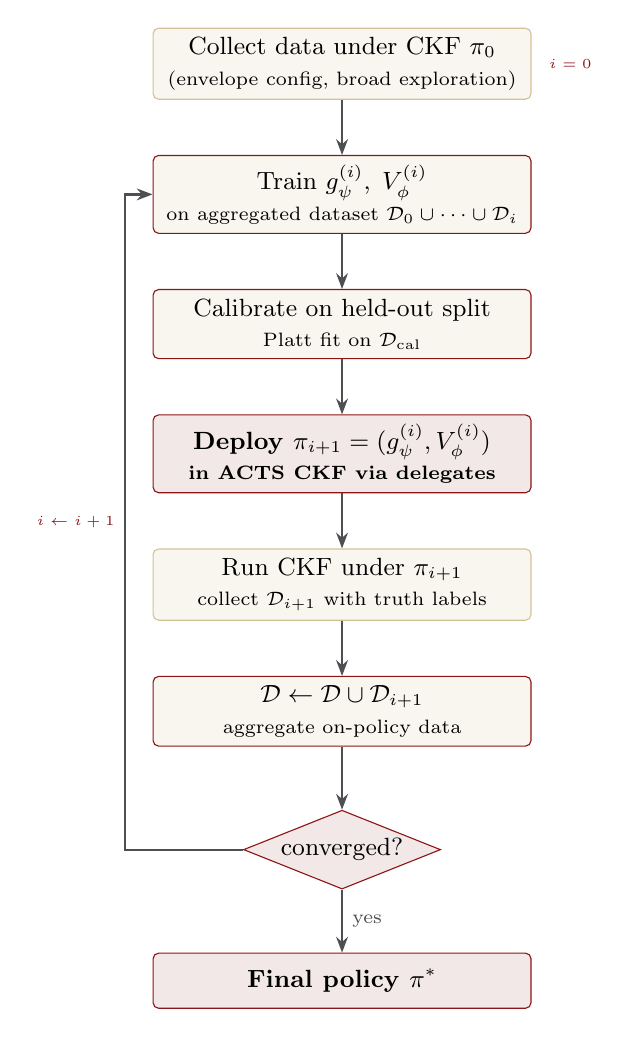
\begin{tikzpicture}[
        node distance=0.7cm,
        mystep/.style={rectangle, draw=cardinal, fill=lightsand,
          minimum width=4.8cm, minimum height=0.7cm,
          rounded corners=2pt, align=center, font=\small},
        policy/.style={rectangle, draw=cardinal, fill=cardinal!10,
          minimum width=4.8cm, minimum height=0.7cm,
          rounded corners=2pt, align=center, font=\small\bfseries},
        data/.style={rectangle, draw=sandstone, fill=sandstone!15,
          minimum width=4.8cm, minimum height=0.7cm,
          rounded corners=2pt, align=center, font=\small},
        decision/.style={diamond, draw=cardinal, fill=cardinal!10,
          minimum width=1.2cm, minimum height=0.8cm,
          align=center, font=\small, inner sep=1pt, aspect=2.5},
        arrow/.style={-{Stealth[length=2mm]}, thick, draw=coolgrey},
        lbl/.style={font=\scriptsize\color{coolgrey}, align=center},
        iter/.style={font=\tiny\itshape\color{cardinal}},
      ]

      % Step 0: Initial data
      \node[data] (d0) {Collect data under CKF $\pi_0$\\
        {\scriptsize (envelope config, broad exploration)}};
      \node[iter, right=0.1cm of d0] {$i=0$};

      % Step 1: Train
      \node[mystep, below=of d0] (train) {Train $g_\psi^{(i)},\; V_\phi^{(i)}$\\
        {\scriptsize on aggregated dataset $\mathcal{D}_0 \cup \cdots \cup \mathcal{D}_i$}};

      % Step 2: Calibrate
      \node[mystep, below=of train] (calib) {Calibrate on held-out split\\
        {\scriptsize Platt fit on $\mathcal{D}_\text{cal}$}};

      % Step 3: Deploy
      \node[policy, below=of calib] (deploy) {Deploy $\pi_{i+1} = (g_\psi^{(i)}, V_\phi^{(i)})$\\
        {\scriptsize in ACTS CKF via delegates}};

      % Step 4: Run on-policy
      \node[data, below=of deploy] (collect) {Run CKF under $\pi_{i+1}$\\
        {\scriptsize collect $\mathcal{D}_{i+1}$ with truth labels}};

      % Step 5: Aggregate
      \node[mystep, below=of collect] (aggregate) {$\mathcal{D} \leftarrow \mathcal{D} \cup \mathcal{D}_{i+1}$\\
        {\scriptsize aggregate on-policy data}};

      % Step 6: Converged?
      \node[decision, below=0.8cm of aggregate] (converge) {converged?};

      % Done
      \node[policy, below=0.8cm of converge] (done) {Final policy $\pi^*$};

      % Arrows
      \draw[arrow] (d0) -- (train);
      \draw[arrow] (train) -- (calib);
      \draw[arrow] (calib) -- (deploy);
      \draw[arrow] (deploy) -- (collect);
      \draw[arrow] (collect) -- (aggregate);
      \draw[arrow] (aggregate) -- (converge);
      \draw[arrow] (converge) -- node[right, lbl] {yes} (done);
      \draw[arrow] (converge.west) -- ++(-1.5, 0)
        % node[above, lbl] {no}
        |- node[iter, near start, left] {$i \leftarrow i+1$} (train.west);

      \end{tikzpicture}
      }%
    \end{column}
\end{columns}
\end{frame}

\section{Results} 
\subsection{Inference Mechanics}

\begin{frame}{cCKF Inference Pipeline}
\centering
\resizebox{!}{0.88\textheight}{%
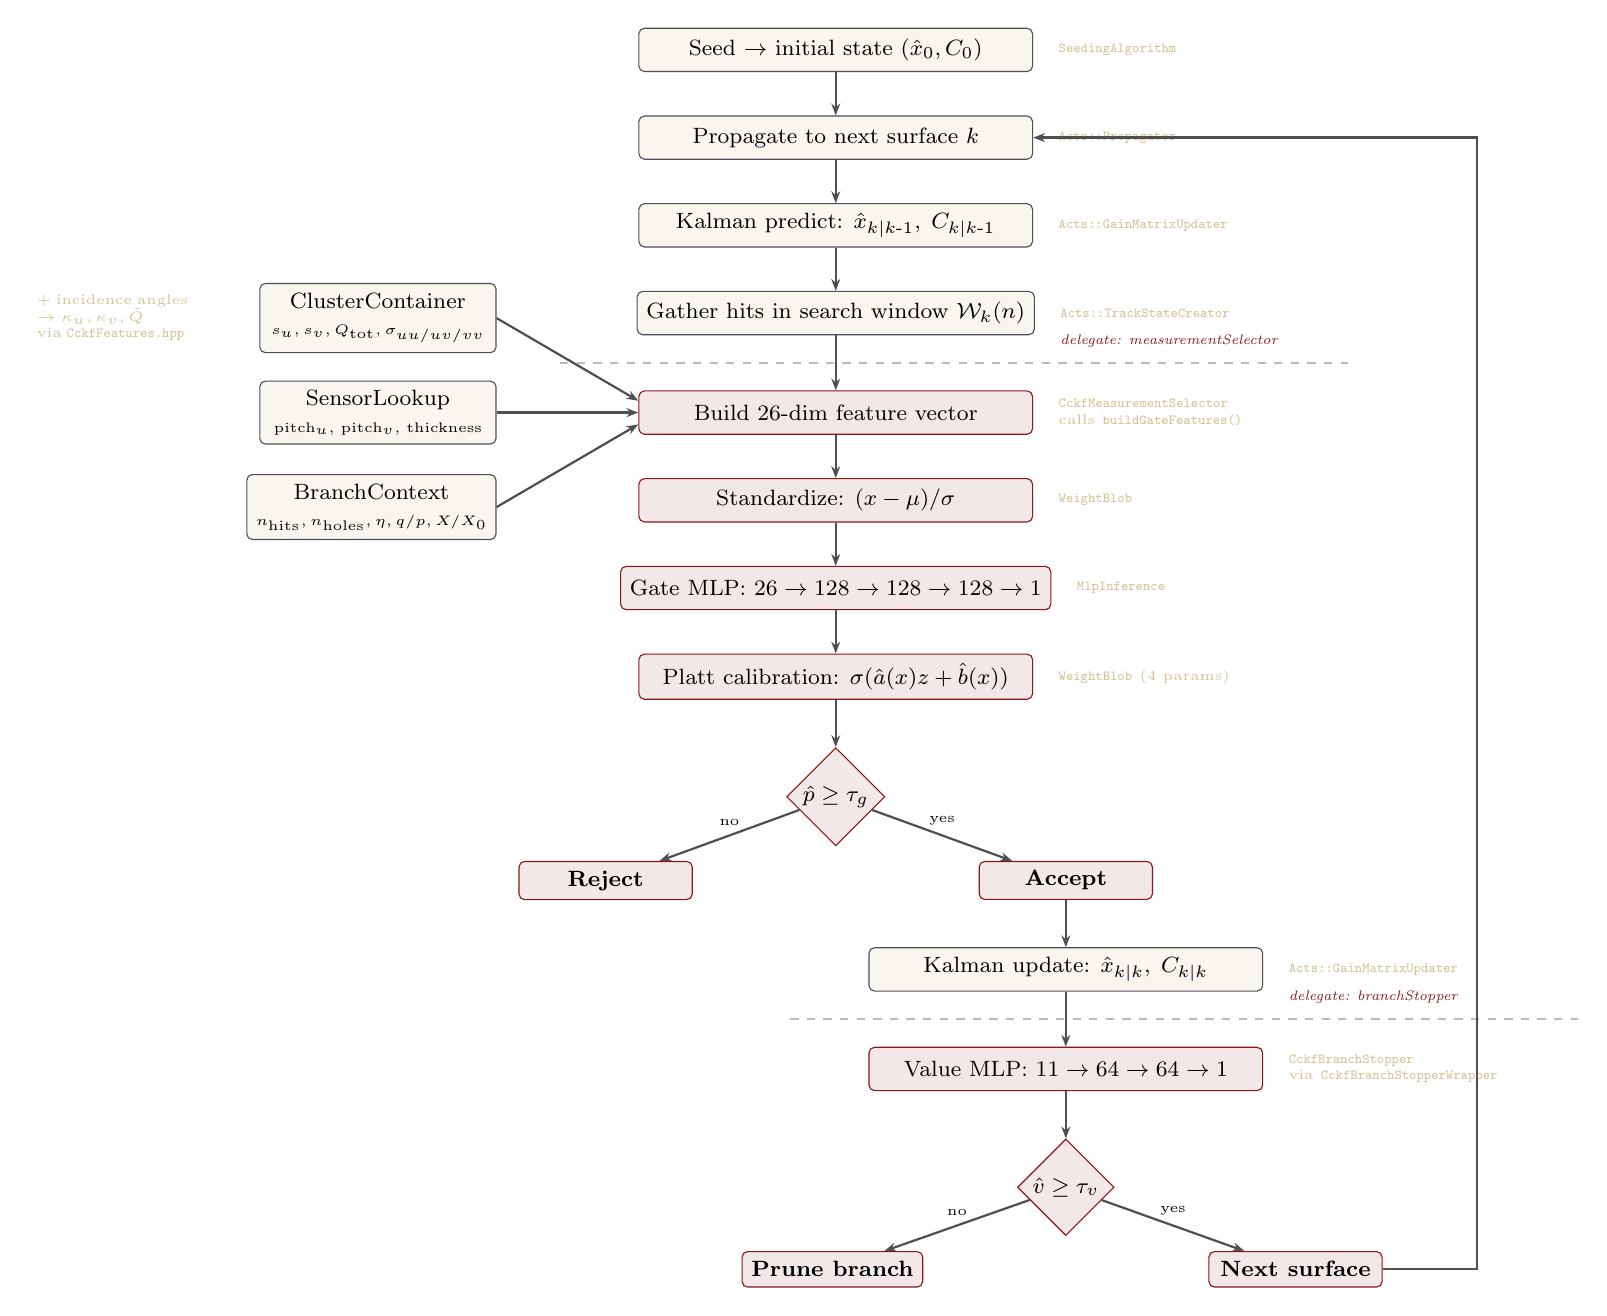
\begin{tikzpicture}[
  node distance=0.55cm,
  acts/.style={rectangle, draw=coolgrey, fill=lightsand,
    minimum width=5cm, minimum height=0.55cm,
    rounded corners=2pt, align=center, font=\footnotesize},
  cckf/.style={rectangle, draw=cardinal, fill=cardinal!10,
    minimum width=5cm, minimum height=0.55cm,
    rounded corners=2pt, align=center, font=\footnotesize},
  decision/.style={diamond, draw=cardinal, fill=cardinal!10,
    minimum width=1cm, minimum height=0.6cm,
    align=center, font=\footnotesize, inner sep=1pt},
  output/.style={rectangle, draw=cardinal, fill=cardinal!10,
    minimum width=2.2cm, minimum height=0.45cm,
    rounded corners=2pt, align=center, font=\footnotesize\bfseries},
  arrow/.style={-{Stealth[length=1.5mm]}, thick, draw=coolgrey},
  class/.style={font=\tiny\ttfamily\color{sandstone}, align=left},
  delegate/.style={font=\tiny\itshape\color{cardinal}, align=right},
  sep/.style={draw=coolgrey!40, dashed, thick},
]

% === ACTS: Seed + Propagate ===
\node[acts] (seed) {Seed $\to$ initial state $(\hat x_0, C_0)$};
\node[class, right=0.2cm of seed] {SeedingAlgorithm};

\node[acts, below=of seed] (propagate) {Propagate to next surface $k$};
\node[class, right=0.2cm of propagate] {Acts::Propagator};

\node[acts, below=of propagate] (predict) {Kalman predict: $\hat x_{k|k\text{-}1},\; C_{k|k\text{-}1}$};
\node[class, right=0.2cm of predict] {Acts::GainMatrixUpdater};

\node[acts, below=of predict] (window) {Gather hits in search window $\mathcal{W}_k(n)$};
\node[class, right=0.2cm of window] {Acts::TrackStateCreator};

% === Delegate insertion: measurementSelector ===
\draw[sep] ([xshift=-3.5cm, yshift=-0.35cm]window.south)
       -- ([xshift=6.5cm, yshift=-0.35cm]window.south);
\node[delegate, right=0.2cm of window, yshift=-0.35cm]
  {\textrm{delegate:} measurementSelector};

% === cCKF: Feature build ===
\node[cckf, below=0.7cm of window] (features) {%
  Build 26-dim feature vector};
\node[class, right=0.2cm of features] {%
  CckfMeasurementSelector\\
  \textrm{calls} buildGateFeatures()};

% Feature inputs (compact, left side)
\node[acts, left=1.8cm of features, yshift=1.2cm, minimum width=3cm]
  (clus_src) {ClusterContainer\\{\tiny $s_u, s_v, Q_\text{tot}, \sigma_{uu/uv/vv}$}};
\node[acts, left=1.8cm of features, yshift=0.0cm, minimum width=3cm]
  (sensor_src) {SensorLookup\\{\tiny pitch$_u$, pitch$_v$, thickness}};
\node[acts, left=1.8cm of features, yshift=-1.2cm, minimum width=3cm]
  (branch_src) {BranchContext\\{\tiny $n_\text{hits}, n_\text{holes}, \eta, q/p, X/X_0$}};

\draw[arrow] (clus_src.east) -- ([yshift=0.15cm]features.west);
\draw[arrow] (sensor_src.east) -- (features.west);
\draw[arrow] (branch_src.east) -- ([yshift=-0.15cm]features.west);

% Derived features annotation
\node[class, left=0.2cm of clus_src, text width=2.5cm] {%
  \textrm{+ incidence angles}\\
  \textrm{$\to \kappa_u, \kappa_v, \tilde Q$}\\
  \textrm{\upshape via} CckfFeatures.hpp};

% === cCKF: Gate MLP ===
\node[cckf, below=of features] (standardize) {%
  Standardize: $(x - \mu) / \sigma$};
\node[class, right=0.2cm of standardize] {WeightBlob};

\node[cckf, below=of standardize] (gate) {%
  Gate MLP: $26 \to 128 \to 128 \to 128 \to 1$};
\node[class, right=0.2cm of gate] {MlpInference};

\node[cckf, below=of gate] (platt) {%
  Platt calibration: $\sigma(\hat a(x) z + \hat b(x))$};
\node[class, right=0.2cm of platt] {WeightBlob \textrm{(4 params)}};

% === Gate decision ===
\node[decision, below=0.6cm of platt] (gate_dec) {$\hat p \geq \tau_g$};

\node[output, below left=0.5cm and 1.5cm of gate_dec] (reject) {Reject};
\node[output, below right=0.5cm and 1.5cm of gate_dec] (accept) {Accept};

% === ACTS: Kalman update ===
\node[acts, below=0.6cm of accept] (update) {%
  Kalman update: $\hat x_{k|k},\; C_{k|k}$};
\node[class, right=0.2cm of update] {Acts::GainMatrixUpdater};

% === Delegate insertion: branchStopper ===
\draw[sep] ([xshift=-3.5cm, yshift=-0.35cm]update.south)
       -- ([xshift=6.5cm, yshift=-0.35cm]update.south);
\node[delegate, right=0.2cm of update, yshift=-0.35cm]
  {\textrm{delegate:} branchStopper};

% === cCKF: Value function ===
\node[cckf, below=0.7cm of update] (value) {%
  Value MLP: $11 \to 64 \to 64 \to 1$};
\node[class, right=0.2cm of value] {%
  CckfBranchStopper\\
  \textrm{via} CckfBranchStopperWrapper};

\node[decision, below=0.6cm of value] (val_dec) {$\hat v \geq \tau_v$};

\node[output, below left=0.5cm and 1.5cm of val_dec] (prune) {Prune branch};
\node[output, below right=0.5cm and 1.5cm of val_dec] (continue) {Next surface};

% === Arrows ===
\draw[arrow] (seed) -- (propagate);
\draw[arrow] (propagate) -- (predict);
\draw[arrow] (predict) -- (window);
\draw[arrow] (window) -- (features);
\draw[arrow] (features) -- (standardize);
\draw[arrow] (standardize) -- (gate);
\draw[arrow] (gate) -- (platt);
\draw[arrow] (platt) -- (gate_dec);
\draw[arrow] (gate_dec) -- node[above, font=\tiny] {no} (reject);
\draw[arrow] (gate_dec) -- node[above, font=\tiny] {yes} (accept);
\draw[arrow] (accept) -- (update);
\draw[arrow] (update) -- (value);
\draw[arrow] (value) -- (val_dec);
\draw[arrow] (val_dec) -- node[above, font=\tiny] {no} (prune);
\draw[arrow] (val_dec) -- node[above, font=\tiny] {yes} (continue);

% Loop back
\draw[arrow] (continue.east) -- ++(1.2,0) |- (propagate.east);

\end{tikzpicture}
}%
\end{frame}

\subsection{Bug Fixes}

\begin{frame}{Two Bugs: NaN in $S_{11}$ and Missing Strips}
  \begin{itemize}
    \item \textbf{$S_{11}$ NaN.} Strip sensors measure one coordinate, so their
      residual covariance is $1\times1$. The feature builder read the full
      $2\times2$ block on every surface. On strips this produced NaN features
      and undefined behavior in Eigen expression proxies, which caused
      segfaults during inference.
    \item \textbf{Fix:} dimension-aware feature extraction, and every Eigen
      accessor result materialized with \texttt{.eval()} before use.
    \item \textbf{The strip bug.} Endcap geometry ids carry a ring index in
      their lowest byte. A join in the data pipeline zeroed that byte, so every
      endcap hit silently dropped out of the training set. The first gate was
      trained on barrel pixels only.
    \item \textbf{Fix:} normalize geometry ids in every loader. All 32 events
      were then re-expanded and every training cache rebuilt.
  \end{itemize}
\end{frame}

\begin{frame}{Distribution Shift at the Selector}
  \begin{columns}
    \begin{column}{0.5\textwidth}
      \begin{figure}
        \centering
        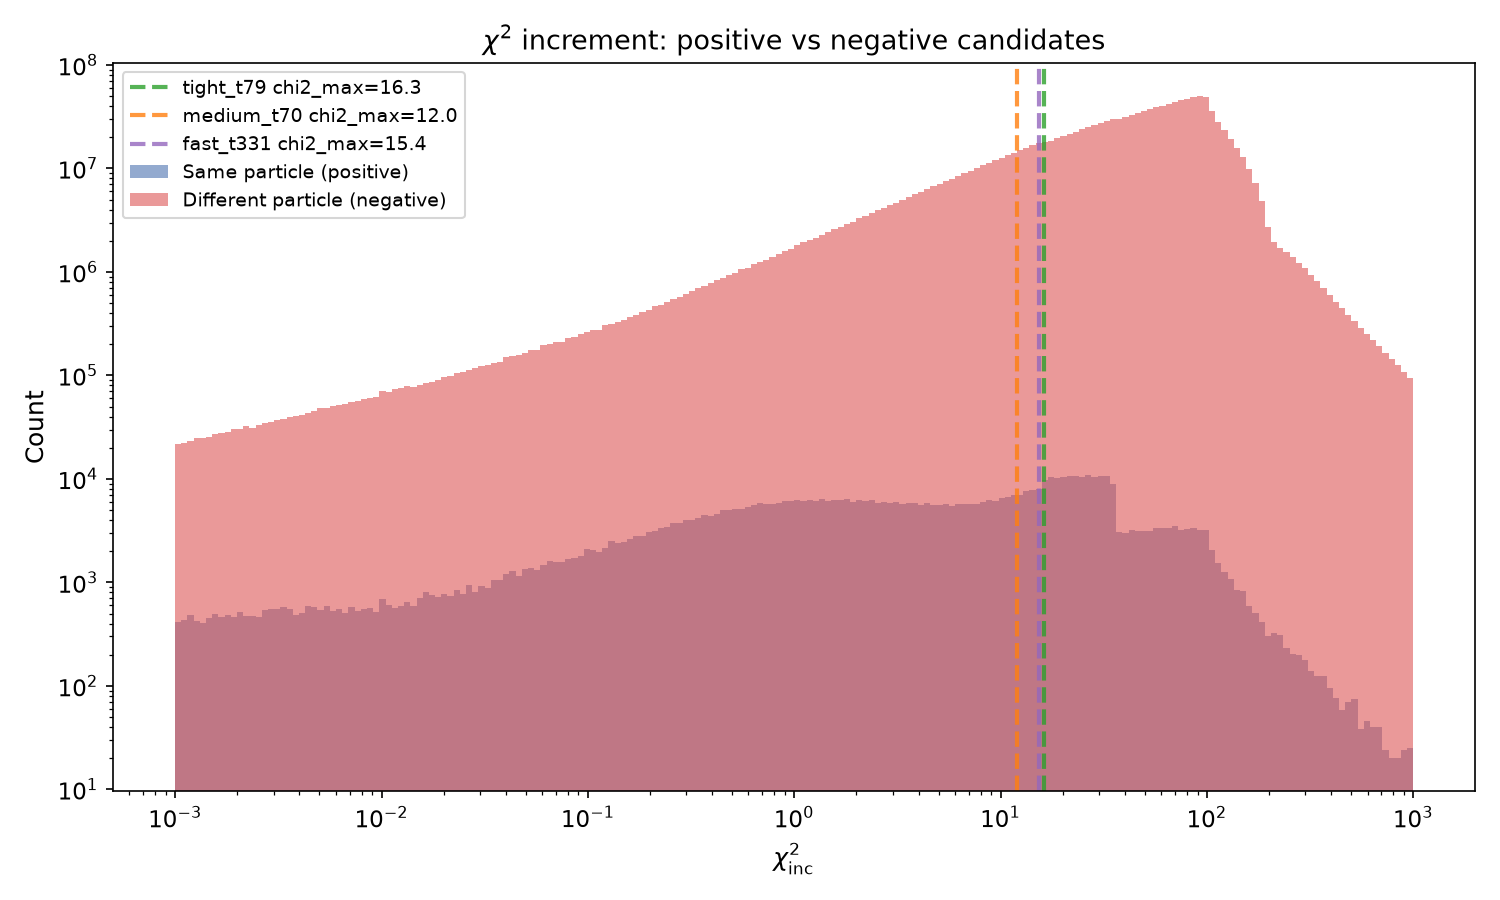
\includegraphics[width=\linewidth]{chi2_training.png}
        \caption{Training: $\chi^2$ increments of gate candidates, with the
          tuned CKF cut values marked.}
      \end{figure}
    \end{column}
    \begin{column}{0.5\textwidth}
      \begin{figure}
        \centering
        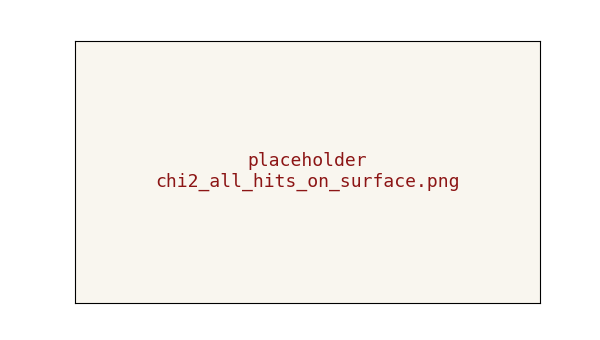
\includegraphics[width=\linewidth]{chi2_all_hits_on_surface.png}
        \caption{Inference: the selector receives every hit on the surface,
          so the $\chi^2$ feature blows up relative to training. Fixed with
          a spatial pre-filter that reproduces the training window.}
      \end{figure}
    \end{column}
  \end{columns}
\end{frame}

\subsection{Retraining}

\begin{frame}{Retraining After the Fixes}
  \begin{itemize}
    \item All four models retrained on the rebuilt caches (full detector,
      endcaps included).
  \end{itemize}
  \vspace{0.2cm}
  \centering
  \begin{tabular}{lrrrr}
    \toprule
    Model & AUC-ROC & AUC-PR & ECE & $\chi^2$ ECE \\
    \midrule
    Gate, majority seeds  & 0.989 & 0.852 & 0.0001 & 0.062 \\
    Gate, pure seeds      & 0.991 & 0.960 & 0.0010 & 0.059 \\
    Value T2, majority    & 0.822 & 0.535 & 0.0025 & -- \\
    Value T2, pure        & 0.940 & 0.972 & 0.0082 & -- \\
    \bottomrule
  \end{tabular}
  \vspace{0.3cm}
  \begin{itemize}
    \item The majority gate is 129$\times$ better calibrated than the $\chi^2$
      likelihood on the same calibration split.
    \item The value function sits 0.056 above the soft-target entropy floor,
      close to the irreducible limit.
  \end{itemize}
\end{frame}

\begin{frame}{Gate Calibration}
  \begin{figure}
    \centering
    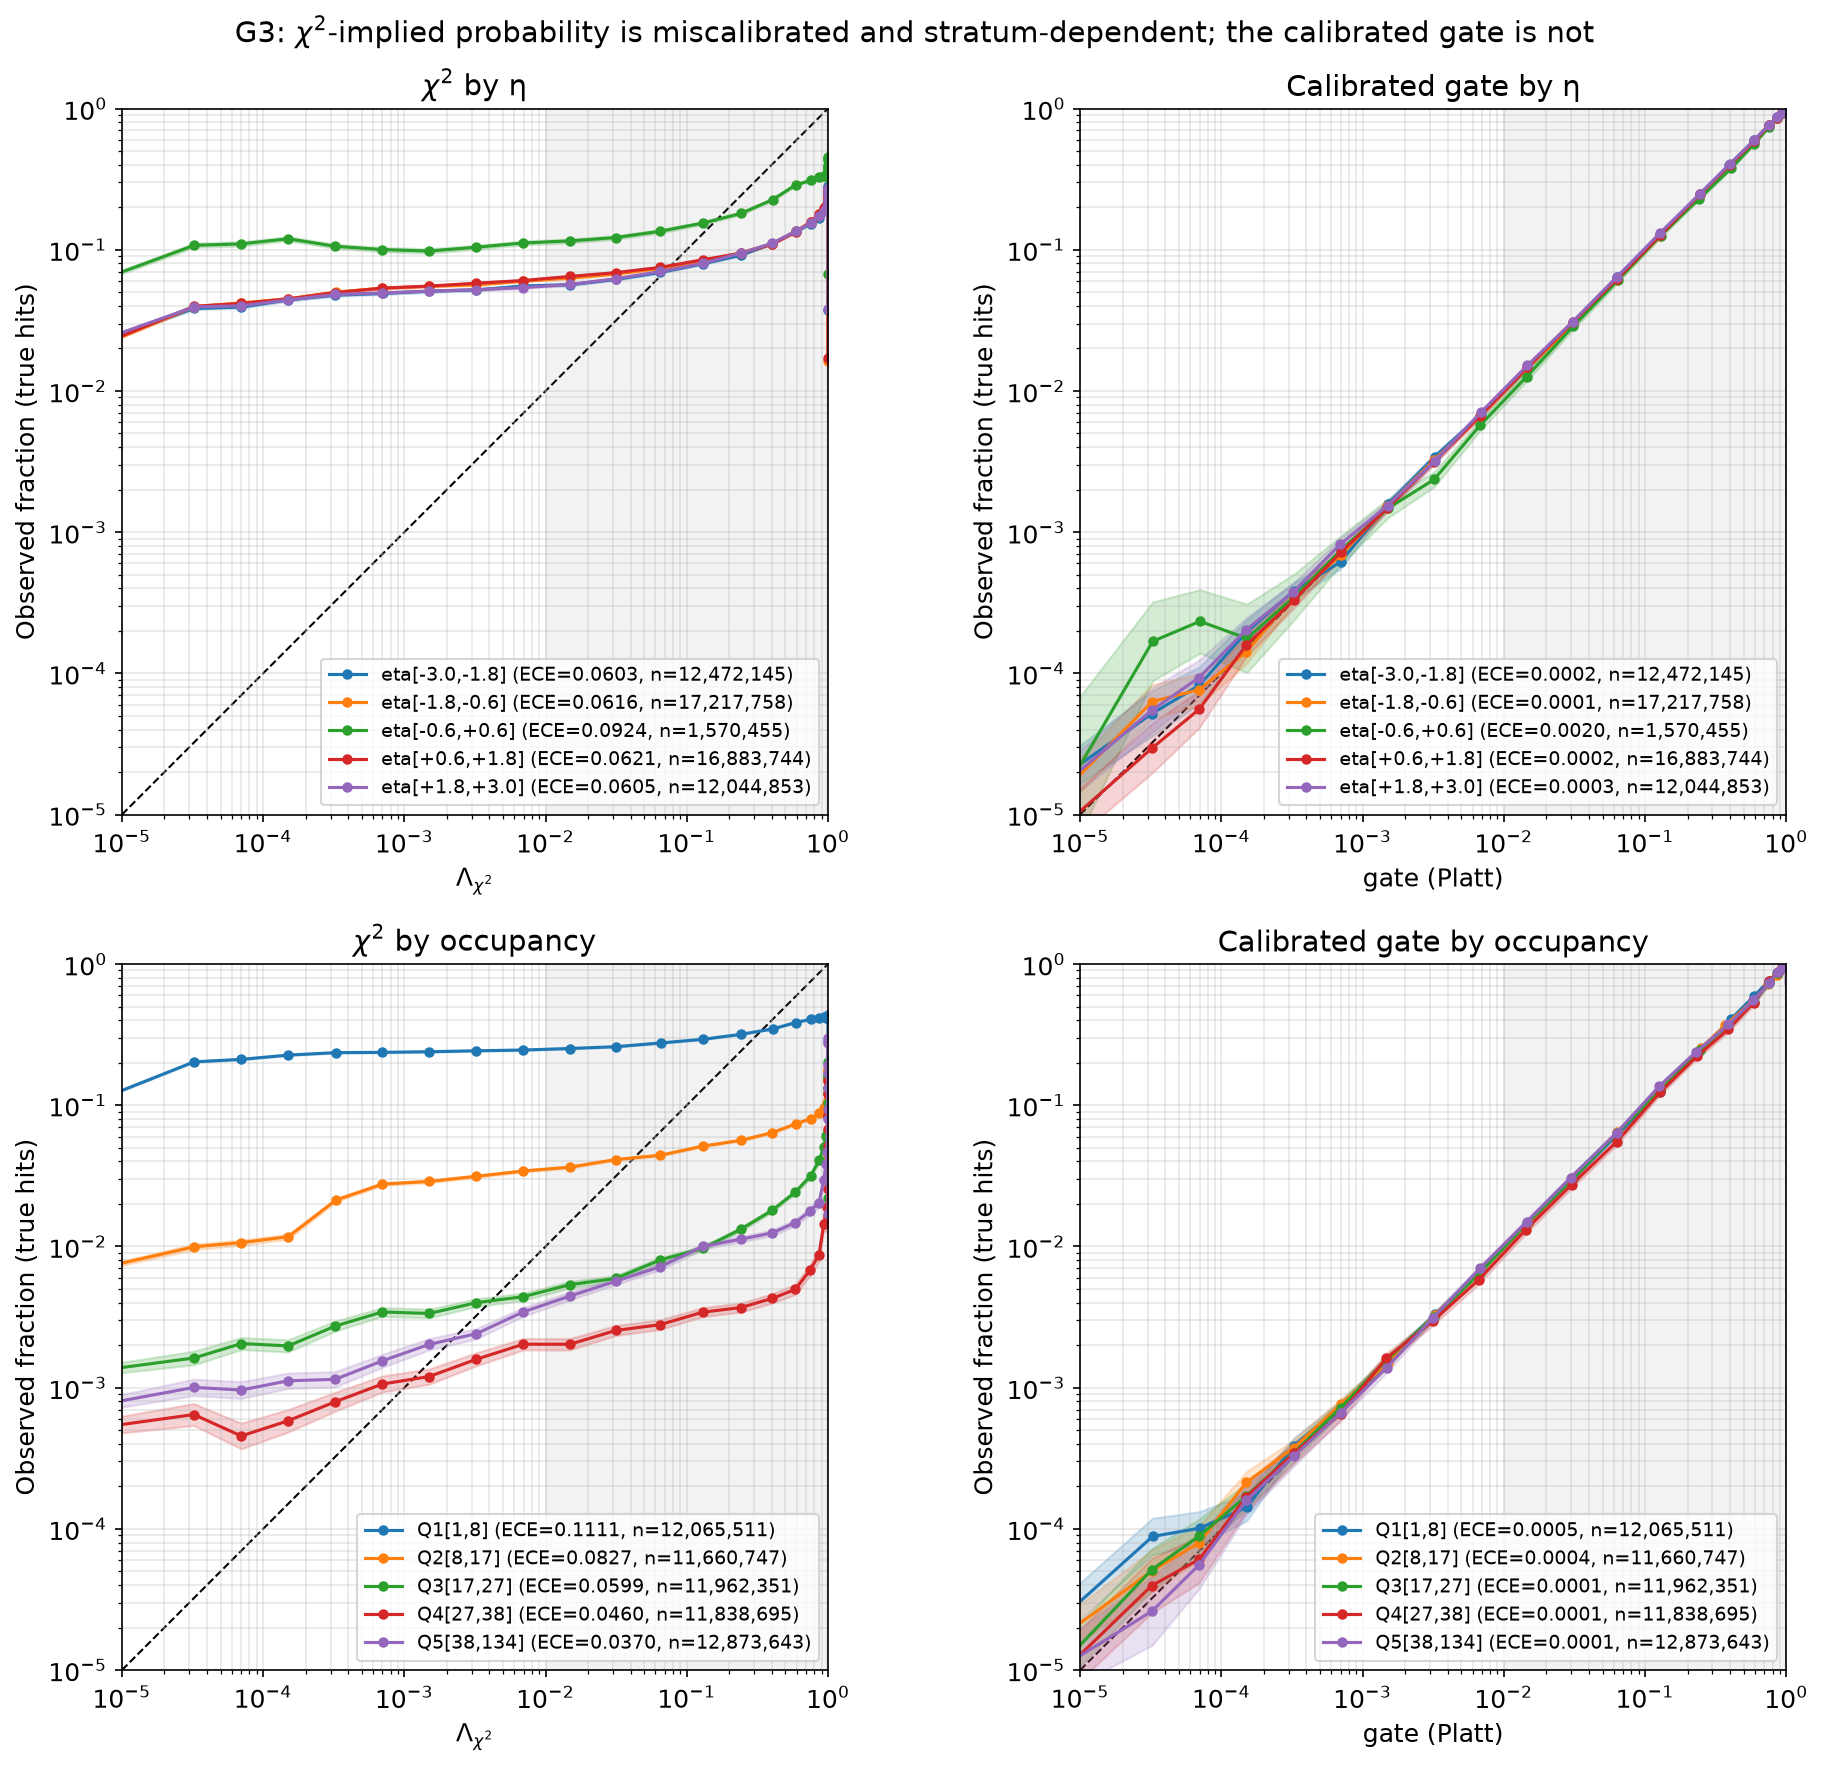
\includegraphics[width=0.62\linewidth]{g3_gate_maj.png}
    \caption{Reliability of the majority-seed gate against the $\chi^2$
      likelihood baseline (calibration split, 40M candidates). The raw network
      is already on the diagonal; Platt correction is a no-op.}
  \end{figure}
\end{frame}

\begin{frame}{Occupancy Adaptation and Value Reliability}
  \begin{columns}
    \begin{column}{0.5\textwidth}
      \begin{figure}
        \centering
        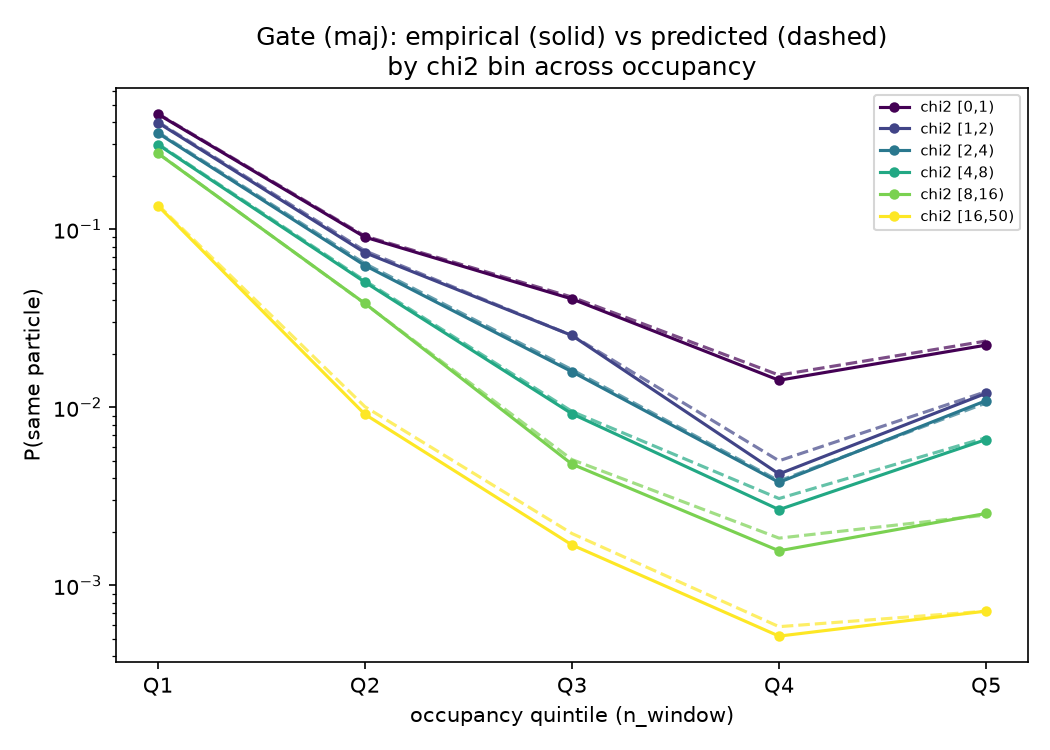
\includegraphics[width=\linewidth]{occupancy_adaptation.png}
        \caption{At fixed $\chi^2$, the true match probability falls
          $\sim$30$\times$ from sparse to dense regions. The gate tracks it.}
      \end{figure}
    \end{column}
    \begin{column}{0.5\textwidth}
      \begin{figure}
        \centering
        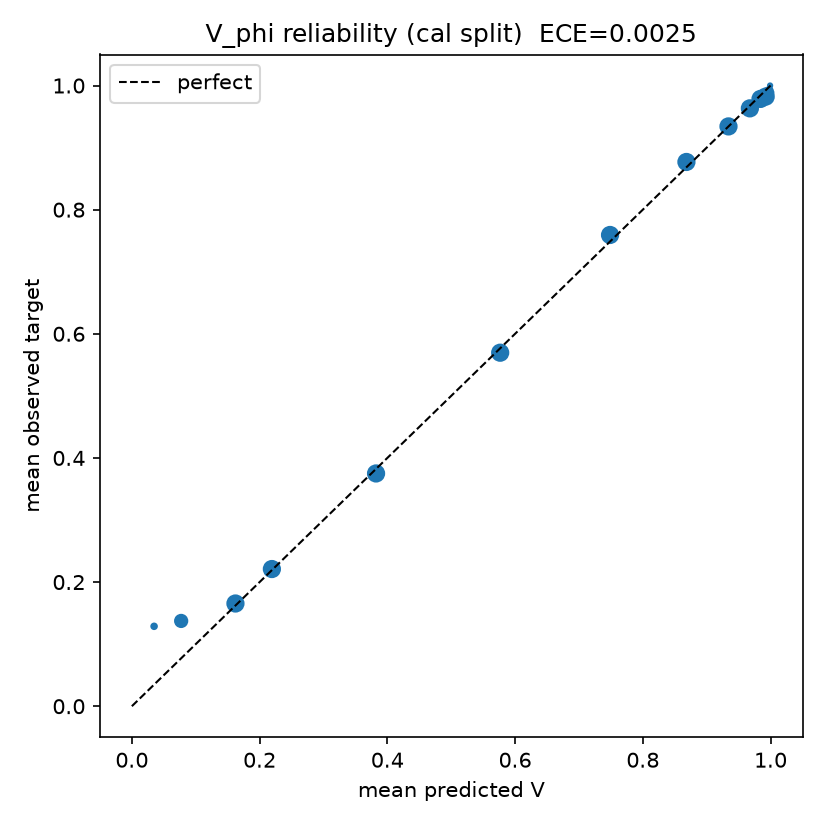
\includegraphics[width=0.85\linewidth]{value_reliability_maj.png}
        \caption{$V_\phi$ reliability on the calibration split (19M branch
          states), ECE 0.0025.}
      \end{figure}
    \end{column}
  \end{columns}
\end{frame}

\subsection{Threshold Grid Search}

\begin{frame}{Grid Search: Pure vs Majority Seeds}
  \begin{columns}
    \begin{column}{0.45\textwidth}
      \begin{itemize}
        \item 12-point grid over $(\tau_g, \tau_v)$ on a validation event,
          for each seed population.
        \item Majority pair: efficiency 0.94 at the loose end against the
          ACTS baseline of 0.37. Fake rate falls from 0.48 to 0.15 as the
          gate tightens, so the threshold behaves as a real likelihood-ratio
          test.
        \item Pure pair: fake rate is flat near 0.85 at every threshold.
      \end{itemize}
    \end{column}
    \begin{column}{0.55\textwidth}
      \begin{figure}
        \centering
        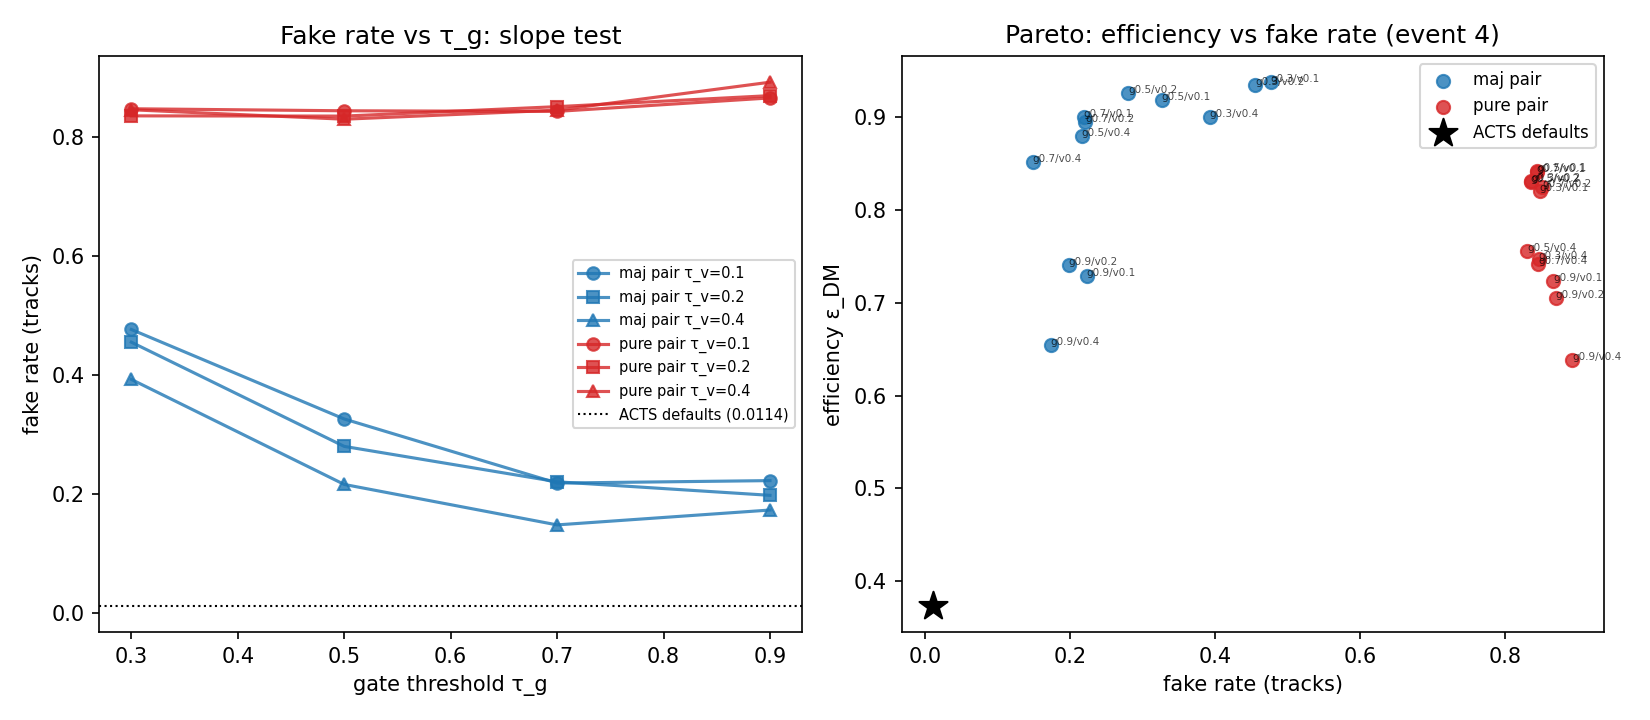
\includegraphics[width=\linewidth]{pareto_maj_vs_pure.png}
      \end{figure}
    \end{column}
  \end{columns}
\end{frame}

\begin{frame}{Interpreting the High Fake Rates}
  \begin{itemize}
    \item The pure models never saw branches from majority seeds during
      training. On those branches their probabilities are meaningless, so
      the threshold stops discriminating and fakes pass at every setting.
      Calibration holds only on the training distribution.
    \item The majority pair responds correctly to its thresholds but its
      absolute fake rate still sits above the baseline. Two reasons:
    \begin{itemize}
      \item The grid is coarse and has not reached the low-fake corner of
        threshold space.
      \item Ambiguity resolution is unchanged from stock ACTS and does not
        yet use the calibrated scores, so fakes that reach it mostly
        survive.
    \end{itemize}
    \item Efficiency more than doubles over the baseline at every grid
      point, so the trade is threshold placement, not model quality.
  \end{itemize}
\end{frame}

\subsection{Tier 3 Value Targets}

\begin{frame}{Tier 3: Value Targets by Re-propagation}
  \begin{itemize}
    \item Tier 3 targets require rolling the CKF forward truth-greedily from
      every branch state. Naively that is one propagation per state, which is
      millions per event.
    \item \textbf{Backward collapse.} Walk each branch backward from its tip.
      Wherever the branch action matches the truth-greedy pick, the value
      follows from the child state by recurrence. Only divergence points and
      tips need a real rollout. This removes 77\% of the propagations.
    \item \textbf{Worklist mechanic.} Each state that needs a rollout is
      written to a worklist row: seed id, step, surface id, bound parameters,
      covariance. A C++ executor seeds the ACTS propagator from each row and
      follows the branch's majority particle to termination, logging the hit
      sequence.
    \item Validated on one event: 419{,}704 of 419{,}704 rollouts completed
      with zero surface lookup failures. Generation for all 32 events is
      queued; target composition and training follow.
  \end{itemize}
\end{frame}

\begin{frame}{Backward Stitching}
  \begin{itemize}
    \item One branch, walked tip to seed. Rollouts run only where they are
      needed; everything else is stitched by recurrence.
  \end{itemize}
  \vspace{0.1cm}
  \centering
  \resizebox{0.92\textwidth}{!}{%
  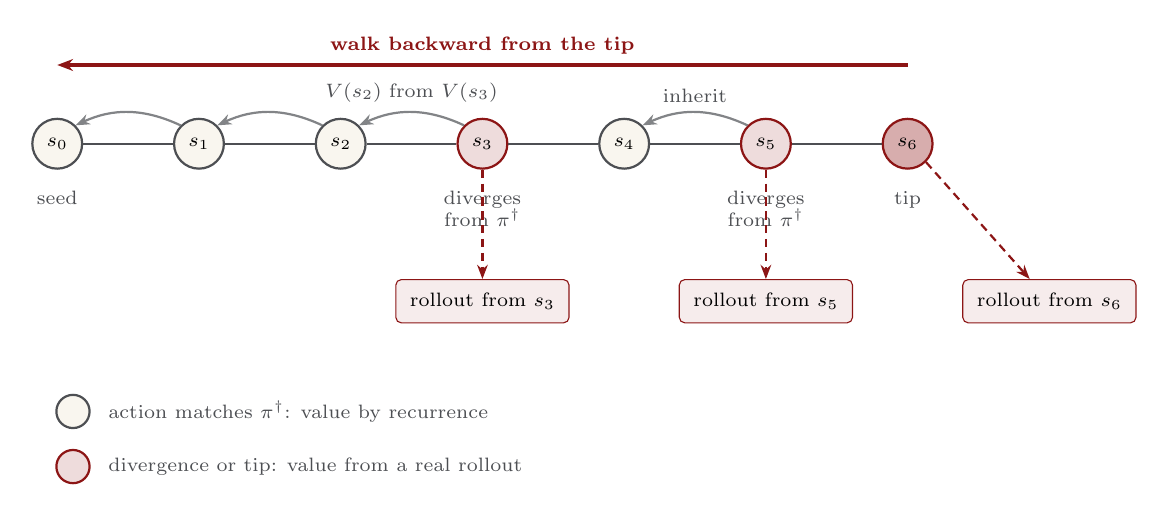
\begin{tikzpicture}[
    state/.style={circle, draw, thick, minimum size=18pt, inner sep=0pt,
      font=\scriptsize\bfseries},
    agree/.style={state, draw=coolgrey, fill=lightsand},
    diverge/.style={state, draw=cardinal, fill=cardinal!15},
    tip/.style={state, draw=cardinal, fill=cardinal!35},
    roll/.style={rectangle, draw=cardinal, fill=cardinal!8,
      rounded corners=2pt, minimum width=2.2cm, minimum height=0.55cm,
      align=center, font=\scriptsize},
    branch/.style={thick, draw=coolgrey},
    back/.style={-{Stealth[length=2mm]}, very thick, draw=cardinal},
    rollarrow/.style={-{Stealth[length=1.8mm]}, thick, draw=cardinal,
      densely dashed},
    inherit/.style={-{Stealth[length=1.8mm]}, thick, draw=coolgrey!70},
    lbl/.style={font=\scriptsize, text=coolgrey, align=center},
    rlbl/.style={font=\scriptsize\bfseries, text=cardinal, align=center},
  ]

    % Branch states, seed (left) to tip (right)
    \node[agree]   (s0) at (0,0)   {$s_0$};
    \node[agree]   (s1) at (1.8,0) {$s_1$};
    \node[agree]   (s2) at (3.6,0) {$s_2$};
    \node[diverge] (s3) at (5.4,0) {$s_3$};
    \node[agree]   (s4) at (7.2,0) {$s_4$};
    \node[diverge] (s5) at (9.0,0) {$s_5$};
    \node[tip]     (s6) at (10.8,0){$s_6$};

    \draw[branch] (s0) -- (s1) -- (s2) -- (s3) -- (s4) -- (s5) -- (s6);

    \node[lbl, below=0.15cm of s0] {seed};
    \node[lbl, below=0.15cm of s3] {diverges\\from $\pi^\dagger$};
    \node[lbl, below=0.15cm of s5] {diverges\\from $\pi^\dagger$};
    \node[lbl, below=0.15cm of s6] {tip};

    % Backward walk arrow
    \draw[back] (10.8,1.0) -- node[above, rlbl] {walk backward from the tip}
      (0,1.0);

    % Rollouts hang off divergence states and the tip
    \node[roll] (r3) at (5.4,-2.0) {rollout from $s_3$};
    \node[roll] (r5) at (9.0,-2.0) {rollout from $s_5$};
    \node[roll] (r6) at (12.6,-2.0) {rollout from $s_6$};
    \draw[rollarrow] (s3) -- (r3);
    \draw[rollarrow] (s5) -- (r5);
    \draw[rollarrow] (s6.south east) -- (r6);

    % Recurrence arrows for agreeing states
    \draw[inherit] (s3.north west) to[bend right=25]
      node[above, lbl] {$V(s_2)$ from $V(s_3)$} (s2.north east);
    \draw[inherit] (s2.north west) to[bend right=25] (s1.north east);
    \draw[inherit] (s1.north west) to[bend right=25] (s0.north east);
    \draw[inherit] (s5.north west) to[bend right=25]
      node[above, lbl] {inherit} (s4.north east);

    % Legend
    \node[agree, minimum size=12pt] (leg1) at (0.2,-3.4) {};
    \node[lbl, right=0.1cm of leg1] {action matches $\pi^\dagger$: value by recurrence};
    \node[diverge, minimum size=12pt] (leg2) at (0.2,-4.1) {};
    \node[lbl, right=0.1cm of leg2] {divergence or tip: value from a real rollout};

  \end{tikzpicture}
  }%
\end{frame}

\subsection{Status}

\begin{frame}{Current Runs}
  \begin{itemize}
    \item \textbf{EHVI Pareto sweeps.} Adaptive threshold search with expected
      hypervolume improvement, warm-started from the grids. Five rounds of
      eight points per seed population, running on Perlmutter.
    \item \textbf{Window scan.} The strongest grid points rerun at search
      window sizes $n \in \{7, 5, 3\}$ to separate the speedup from shrinking
      the window from the accuracy cost of leaving its training value.
    \item \textbf{Tier 3 generation.} Worklist and rollout jobs for all 32
      events.
    \item \textbf{DAgger data.} Every sweep run logs its track states, so
      on-policy training data accumulates for free.
  \end{itemize}
\end{frame}

\section{Further Work}

\begin{frame}{Next Week}
  \begin{itemize}
    \item Finish EHVI Pareto fronts for all four pairs: gate $\times$
      \{majority, pure\} with value tier 2, then tier 3.
    \item Train and benchmark both tier 3 value functions against tier 2.
    \item Make the DAgger call: measure calibration drift on the logged
      on-policy states. Iterate only if the drift is material.
    \item Use the calibrated scores in ambiguity resolution and remeasure
      the fake rate.
  \end{itemize}
\end{frame}

\end{document}
